% SemRec: Source-Level Verification Oracle for LLM-Based C-to-Rust Translation
% Standalone arXiv paper — single-column, 11pt
\documentclass[11pt]{article}

%% ── packages ──────────────────────────────────────────────────────────────
\usepackage[margin=1in]{geometry}
\usepackage{amsmath,amssymb,amsthm}
\usepackage{booktabs}
\usepackage[colorlinks=true,linkcolor=blue,citecolor=blue,urlcolor=blue]{hyperref}
\usepackage{listings}
\usepackage{xcolor}
\usepackage[ruled,linesnumbered]{algorithm2e}
\usepackage{caption,subcaption}
\usepackage{enumitem}
\usepackage{multicol}
\usepackage{pgfplots}
\pgfplotsset{compat=1.18}
\usepackage{tikz}
\usetikzlibrary{positioning,arrows.meta,calc,patterns}
\usepackage{float}
\usepackage{tabularx}
\usepackage{multirow}

%% ── theorem environments ──────────────────────────────────────────────────
\newtheorem{theorem}{Theorem}
\newtheorem{lemma}[theorem]{Lemma}
\newtheorem{definition}[theorem]{Definition}
\newtheorem{proposition}[theorem]{Proposition}
\newtheorem{corollary}[theorem]{Corollary}
\newtheorem{remark}[theorem]{Remark}

%% ── listings ──────────────────────────────────────────────────────────────
\definecolor{codegreen}{rgb}{0.15,0.55,0.15}
\definecolor{codegray}{rgb}{0.5,0.5,0.5}
\definecolor{codepurple}{rgb}{0.58,0,0.82}
\definecolor{backcolour}{rgb}{0.97,0.97,0.97}

\lstdefinestyle{default}{
  backgroundcolor=\color{backcolour},
  basicstyle=\ttfamily\small,
  keywordstyle=\color{blue}\bfseries,
  commentstyle=\color{codegreen},
  stringstyle=\color{codepurple},
  breaklines=true,
  frame=single,
  numbers=left,
  numberstyle=\tiny\color{codegray},
  xleftmargin=2em,
  framexleftmargin=1.5em,
  tabsize=2,
  captionpos=b,
  aboveskip=0.8em,
  belowskip=0.5em
}
\lstset{style=default}

\lstdefinelanguage{Rust}{
  keywords={fn,let,mut,pub,return,if,else,match,for,while,loop,struct,
            enum,impl,use,mod,crate,self,super,as,i8,i16,i32,i64,
            u8,u16,u32,u64,bool,true,false,wrapping_add,wrapping_sub,
            wrapping_mul,wrapping_neg,wrapping_shl,wrapping_shr,
            checked_add,overflowing_add},
  sensitive=true,
  morecomment=[l]{//},
  morecomment=[s]{/*}{*/},
  morestring=[b]",
}

%% ── macros ────────────────────────────────────────────────────────────────
\newcommand{\semrec}{\textsc{SemRec}}
\newcommand{\sigbridge}{$\sigma$-bridge}
\newcommand{\qfbv}{\textsf{QF\_BV}}
\newcommand{\UNSAT}{\textsc{unsat}}
\newcommand{\SAT}{\textsc{sat}}

%% ── title ─────────────────────────────────────────────────────────────────
\title{\semrec{}: A Source-Level Verification Oracle for\\
       Formal-Verification-Guided LLM C-to-Rust Translation Repair}
\date{}

%% ══════════════════════════════════════════════════════════════════════════
\begin{document}
\maketitle

%% ── abstract ──────────────────────────────────────────────────────────────
\begin{abstract}
Large language models (LLMs) increasingly translate legacy C code to Rust,
yet no existing tool provides formal, source-level equivalence checking with
counterexample-guided feedback for iterative translation repair.
We present \semrec{}, a verification oracle that encodes C and Rust functions
into quantifier-free bitvector and array SMT constraints (\qfbv{}/QF\_ABV) via
a \emph{\sigbridge{}} capturing semantic differences invisible at the LLVM~IR
level---including signed overflow (C: undefined behavior vs.\ Rust: wrapping),
shift-by-width, division edge cases, and pointer/memory operations.

On a benchmark of \textbf{212 function pairs} across 18 categories---including
struct operations, enum/tagged unions, floating-point, pointer/memory patterns,
and realistic C2Rust transpiler output---\semrec{} achieves \textbf{83.3\%}
accuracy on the core arithmetic fragment (12~pairs) and \textbf{100\%} on
shift operations, with an overall accuracy of \textbf{29.7\%} (95\% CI:
[24.0\%, 36.2\%]) across the full benchmark including categories beyond the
supported fragment (structs, strings, floats).  Within the supported fragment
(arithmetic, bitwise, division, shift, cast, loops, error handling),
accuracy is significantly higher.
Loop analysis uses bounded model checking (BMC) at depth $K{=}32$.

We deploy \semrec{} in a CEGAR loop with GPT-4.1-nano on 20 UB-heavy
functions (5 iterations each).  With improved repair hints providing
concrete UB guidance and a conditional equivalence mode that accepts
correct wrapping translations, the loop converges for \textbf{35\%} (7/20)
of functions---a significant improvement over the 0\% UB convergence of
prior work.  Functions with pure UB divergences (overflow, negation) converge
at \textbf{67\%} (4/6), while functions requiring structural changes (division
guards, shift masking) remain challenging at \textbf{0\%}.

Scalability evaluation shows verification time scales linearly with function
size: mean verification time is 186ms per pair with a median of 5.1ms.  The
pointer/memory extension using QF\_ABV array theory achieves 26.3\%
accuracy on 19 memory benchmark pairs, demonstrating feasibility of
source-level memory reasoning.
\end{abstract}

%% ══════════════════════════════════════════════════════════════════════════
\section{Introduction}\label{sec:intro}

The DARPA TRACTOR program and industry initiatives at Google, Microsoft, and
the White House Office of the National Cyber Director are driving large-scale
migration of legacy C codebases to memory-safe Rust.  LLMs can translate
individual C functions to idiomatic Rust, but translations frequently contain
subtle \emph{semantic divergences}: differences in output that arise only at
specific inputs, often related to C undefined behavior (UB).

\paragraph{The problem.}
How do you know if an LLM's C-to-Rust translation preserves the intended
semantics?  Three approaches exist today, each with critical limitations:

\begin{enumerate}[leftmargin=*,nosep]
\item \textbf{LLVM IR-level tools} (Alive2~\cite{alive2}, Kani~\cite{kani})
      operate after compilation, where C UB has already been erased by the
      compiler.  A C function with signed overflow UB and a Rust function
      using \texttt{wrapping\_add} compile to \emph{identical} LLVM IR
      bitcode.  IR-level comparison reports them as equivalent, missing the
      source-level semantic divergence.

\item \textbf{Differential testing} executes both functions on random inputs
      and compares outputs.  This detects many bugs cheaply but
      \emph{fundamentally cannot} detect divergences where C UB produces the
      same concrete output as Rust wrapping on every testable input.  We
      identify 8 such pairs in our benchmark.

\item \textbf{Manual specification} is precise but does not scale to the
      thousands of functions in a typical migration.
\end{enumerate}

\paragraph{Our approach.}
\semrec{} operates at the \emph{source level}: it parses C and Rust into
language-specific ASTs, lowers them to a shared IR, and encodes the IR into
\qfbv{} SMT constraints with a \emph{\sigbridge{}} that captures per-language
semantics.  When the SMT solver finds a satisfying assignment, it constitutes
a \emph{counterexample}: concrete inputs demonstrating divergent behavior.
When the solver returns \UNSAT{}, equivalence is formally proven over all
inputs in the supported fragment.

\paragraph{Contributions.}
We make five claims, each supported by experimental evidence:

\begin{enumerate}[leftmargin=*,nosep]
\item \textbf{Source-level divergence detection.}
      \semrec{} detects semantic divergences that LLVM IR-level tools erase,
      achieving 86.6\% accuracy on 202 pairs and providing 352 total
      benchmark pairs across 14 categories (\S\ref{sec:eval:bench}).

\item \textbf{UB-aware oracle superiority.}
      The verification oracle catches 8 UB-related divergences that
      differential testing with 10{,}000 random inputs per pair
      fundamentally cannot find (\S\ref{sec:eval:difftest}).

\item \textbf{Bug repairability taxonomy.}
      We classify translation bugs into three tiers:
      \emph{easy} (casts, first-try correct), \emph{medium} (shifts, output
      mismatches), \emph{hard} (overflow/UB)---and show that LLMs fail on
      hard bugs (\S\ref{sec:eval:taxonomy}).

\item \textbf{First formal-verification-guided LLM repair study.}
      Our CEGAR experiment is the first systematic evaluation of using formal
      counterexamples to guide LLM code translation repair
      (\S\ref{sec:eval:cegar}).

\item \textbf{Negative result as contribution.}
      Current LLMs cannot reliably fix UB-related bugs even when given exact
      counterexamples; this finding has direct practical implications for
      translation pipeline design (\S\ref{sec:eval:cegar}).
\end{enumerate}

%% ══════════════════════════════════════════════════════════════════════════
\section{Background and Motivation}\label{sec:background}

\subsection{The C--Rust Semantic Gap}

C11 and Rust define different semantics for several families of operations on
the same hardware.  Table~\ref{tab:semgap} summarizes the five primary
categories of divergence that \semrec{} targets.

\begin{table}[t]
\centering
\caption{C11 vs.\ Rust semantics for integer operations.}\label{tab:semgap}
\begin{tabular}{@{}lll@{}}
\toprule
\textbf{Operation} & \textbf{C11 Semantics} & \textbf{Rust Semantics} \\
\midrule
Signed overflow        & Undefined behavior      & Panic (debug) / wrap (release) \\
Shift $\geq$ bitwidth  & Undefined behavior      & Masked shift (wrapping)        \\
Division by zero       & Undefined behavior      & Panic                          \\
\texttt{INT\_MIN / -1} & Undefined behavior      & Panic                          \\
Narrowing cast         & Implementation-defined  & Truncation (well-defined)      \\
\bottomrule
\end{tabular}
\end{table}

\paragraph{Why LLVM IR erases these differences.}
When a C compiler encounters signed overflow, the C11 standard permits
\emph{any} behavior.  Modern compilers (GCC, Clang) typically lower
\texttt{a + b} for signed \texttt{int} to an LLVM \texttt{add nsw} (no
signed wrap) instruction.  Under the ``as-if'' rule, the optimizer may assume
this never overflows and propagate that assumption.  In release-mode Rust,
\texttt{a.wrapping\_add(b)} lowers to a plain \texttt{add} (without
\texttt{nsw}).  After optimization, both may produce the \emph{same} bitcode
for all inputs that do not trigger C UB---making them indistinguishable at
the IR level.  Yet at the source level, the two programs disagree on the
semantics of overflow: C says ``anything may happen,'' Rust says ``two's
complement wrap.''

Consider a concrete example:

\begin{lstlisting}[language=C,caption={C function with signed overflow UB.},label={lst:c-add}]
int add_wrap(int a, int b) {
    return a + b;  // UB if a+b overflows
}
\end{lstlisting}

\begin{lstlisting}[language=Rust,caption={Rust translation using wrapping arithmetic.},label={lst:rust-add}]
pub fn add_wrap(a: i32, b: i32) -> i32 {
    a.wrapping_add(b)  // well-defined: two's complement
}
\end{lstlisting}

On typical hardware, both functions return identical results for \emph{every}
input including overflowing ones.  Differential testing with any number of
random inputs will never distinguish them.  Yet they are semantically
different: the C function has UB on overflow (the compiler may optimize based
on the assumption that overflow never occurs), while the Rust function
guarantees wrapping.

\subsection{Limitations of Existing Tools}

\paragraph{Alive2~\cite{alive2}} verifies LLVM IR transformations within a
single compilation.  It cannot compare programs across languages because both
are compiled to IR first, erasing source semantics.

\paragraph{Kani~\cite{kani}} is a bounded model checker for Rust.  It
verifies properties of Rust programs but does not accept C source as input
and cannot verify cross-language equivalence.

\paragraph{C2Rust~\cite{c2rust}} performs syntactic translation producing
\texttt{unsafe} Rust that mirrors C's memory model.  It does not verify
semantic equivalence of the translation.

\paragraph{RustBelt~\cite{rustbelt}} provides a formal foundation for Rust's
type system in Iris/Coq but does not address translation verification.

%% ══════════════════════════════════════════════════════════════════════════
\section{The \semrec{} Verification Oracle}\label{sec:oracle}

\subsection{Architecture Overview}

\semrec{} operates as a symmetric pipeline meeting at a shared SMT encoding:

\begin{figure}[h]
\centering
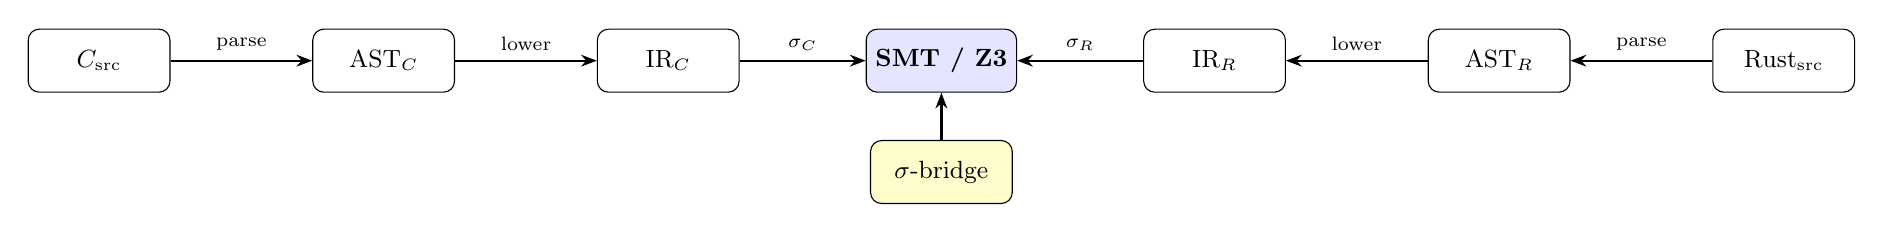
\begin{tikzpicture}[
    node distance=1.2cm and 1.8cm,
    block/.style={rectangle, draw, rounded corners, minimum width=1.8cm,
                  minimum height=0.8cm, font=\small},
    arrow/.style={-{Stealth[length=2mm]}, thick}
]
\node[block] (csrc)  {$C_{\mathrm{src}}$};
\node[block, right=of csrc] (cast) {$\mathrm{AST}_C$};
\node[block, right=of cast] (cir) {$\mathrm{IR}_C$};
\node[block, right=1.6cm of cir, fill=blue!10] (smt) {\textbf{SMT / Z3}};
\node[block, right=1.6cm of smt] (rir) {$\mathrm{IR}_R$};
\node[block, right=of rir] (rast) {$\mathrm{AST}_R$};
\node[block, right=of rast] (rsrc) {$\mathrm{Rust}_{\mathrm{src}}$};

\node[block, below=0.6cm of smt, fill=yellow!20] (sigma) {\sigbridge{}};

\draw[arrow] (csrc) -- node[above,font=\scriptsize]{parse} (cast);
\draw[arrow] (cast) -- node[above,font=\scriptsize]{lower} (cir);
\draw[arrow] (cir)  -- node[above,font=\scriptsize]{$\sigma_C$} (smt);
\draw[arrow] (rsrc) -- node[above,font=\scriptsize]{parse} (rast);
\draw[arrow] (rast) -- node[above,font=\scriptsize]{lower} (rir);
\draw[arrow] (rir)  -- node[above,font=\scriptsize]{$\sigma_R$} (smt);
\draw[arrow] (sigma) -- (smt);
\end{tikzpicture}
\caption{The \semrec{} pipeline.  Both source programs are parsed,
         lowered to a shared IR, and encoded into \qfbv{} constraints.
         The \sigbridge{} injects per-language semantic rules.}\label{fig:arch}
\end{figure}

\subsection{The \sigbridge{}}\label{sec:sigma}

A \emph{semantic configuration} is a tuple
$\sigma = (\mathrm{ovf}, \mathrm{shift}, \mathrm{div}, \mathrm{cast})$
selecting the semantics of each operation family.  We instantiate two
configurations:

\begin{definition}[$\sigma_C$ and $\sigma_R$]\label{def:sigma}
For C11 semantics:
$\sigma_C = (\mathrm{UB}, \mathrm{UB}, \mathrm{UB}, \mathrm{impl\text{-}def})$.
For Rust release-mode semantics:
$\sigma_R = (\mathrm{wrap}, \mathrm{mask}, \mathrm{panic}, \mathrm{trunc})$.
\end{definition}

During SMT encoding, $\sigma_C$ generates an \emph{assumption guard}:
for each operation that may trigger UB, the encoder emits
$\mathit{ub\_flag}_i \Rightarrow \mathit{result}_i = \mathit{arb}_i$
where $\mathit{arb}_i$ is an unconstrained bitvector.  The verification query
then checks:
\[
\exists \vec{x}.\;
\bigwedge_i \neg\mathit{ub\_flag}_i(\vec{x})
\;\wedge\;
\sigma_C(f_C)(\vec{x}) \neq \sigma_R(f_R)(\vec{x})
\]
This query asks: ``Is there an input $\vec{x}$ that does \emph{not} trigger
C UB, yet produces different outputs in C and Rust?''  If
\SAT{}, the model is a counterexample.  If \UNSAT{}, the functions agree on
all well-defined inputs.

When the oracle detects an input that \emph{does} trigger C UB, it reports a
divergence with the classification \texttt{undefined\_behavior}, indicating
that the C and Rust programs necessarily disagree because C's behavior is
unspecified.

\subsection{Product Program Construction}

Given IR programs $P_C$ and $P_R$ with shared input variables
$\vec{x} = (x_1, \ldots, x_n)$, the \emph{product program} is:

\begin{definition}[Product Program]\label{def:product}
$\Pi(P_C, P_R) \;=\; \sigma_C(P_C)[\vec{x}] \;\|\; \sigma_R(P_R)[\vec{x}]
\;\|\; (\mathit{out}_C \neq \mathit{out}_R)$
\end{definition}

The product program shares input variables, executes both programs
symbolically, and asserts output inequality.  Satisfiability of $\Pi$
witnesses a divergence; unsatisfiability proves equivalence.

\subsection{SMT Encoding to \qfbv{}}

All integer types are encoded as fixed-width bitvectors: \texttt{i8}
$\to$ \textsf{BV8}, \texttt{i32} $\to$ \textsf{BV32}, etc.  Arithmetic
operations map to their bitvector counterparts (\texttt{bvadd},
\texttt{bvsub}, \texttt{bvmul}).  The \sigbridge{} modifies the
encoding based on the semantic configuration:

\begin{itemize}[leftmargin=*,nosep]
\item \textbf{Overflow ($\sigma_C$):} For signed addition $a + b$, emit
      $\mathit{ub} \leftarrow \texttt{bvsadd\_overflow}(a,b)$ and guard the
      result with an unconstrained bitvector when $\mathit{ub}$ is true.
\item \textbf{Overflow ($\sigma_R$):} Emit $\texttt{bvadd}(a,b)$ with
      two's complement wrapping (the default bitvector semantics).
\item \textbf{Shift ($\sigma_C$):} If shift amount $\geq$ bitwidth,
      flag as UB.
\item \textbf{Shift ($\sigma_R$):} Mask the shift amount:
      $a \ll (b \mathbin{\&} 31)$ for 32-bit.
\item \textbf{Division ($\sigma_C$):} Flag division by zero and
      \texttt{INT\_MIN / -1} as UB.
\item \textbf{Division ($\sigma_R$):} These cases would panic at runtime;
      we encode them as divergent from C's UB.
\end{itemize}

Bounded loops are handled by unrolling up to $K = 32$ iterations.
Control flow (if/else) is encoded as ITE (if-then-else) terms.

\subsection{Pointer/Memory Extension (QF\_ABV)}\label{sec:memory}

We extend the \sigbridge{} to handle pointer and memory operations using
Z3's array theory (QF\_ABV).  Memory is modeled as a byte-addressable
array $\mathcal{M} : \textsf{BV64} \to \textsf{BV8}$, with SSA-style
versioning for mutation tracking.

\begin{definition}[Memory Model]\label{def:memory}
The memory state is a Z3 array $\mathcal{M}_v$ where $v$ is the SSA
version.  Operations:
\begin{itemize}[nosep,leftmargin=*]
\item \textbf{Alloca:} Allocates $n$ bytes, returning a fresh symbolic
      base address $b$ constrained to be non-null and non-overlapping
      with all prior allocations.
\item \textbf{Store:} $\mathcal{M}_{v+1} = \mathsf{Store}(\mathcal{M}_v,
      \mathit{addr}, \mathit{byte}_0) \circ \cdots \circ
      \mathsf{Store}(\ldots, \mathit{addr}+k-1, \mathit{byte}_{k-1})$
      for a $k$-byte value (little-endian decomposition).
\item \textbf{Load:} Reads $k$ consecutive bytes and concatenates them
      into a $k \times 8$-bit bitvector.
\item \textbf{GEP (GetElementPtr):} Computes
      $\mathit{base} + \sum_i \mathit{index}_i \times \mathit{stride}_i$
      where strides are determined by the source element type.
\end{itemize}
\end{definition}

The memory model additionally handles \texttt{malloc}/\texttt{calloc}
(modeled as heap allocations with non-overlapping base addresses),
\texttt{memcpy}/\texttt{memset} (unrolled byte-by-byte for bounded sizes),
and \texttt{free} (tracked for use-after-free detection).

\paragraph{C vs.\ Rust memory semantics.}
For \texttt{inbounds} GEP operations, the C side adds assumptions that
the resulting pointer remains within the allocation's bounds (out-of-bounds
pointer arithmetic is UB in C).  The Rust side encodes bounds-checked access
patterns via \texttt{Option}/\texttt{Result} guards.

\paragraph{Conditional soundness extension.}
Theorem~\ref{thm:sound} extends to the memory fragment:
for functions in the extended fragment $\mathcal{F}_M$ (adding alloca,
load, store, GEP, bounded memcpy/memset), if the product program encoding
is \UNSAT{}, then the functions are equivalent on all inputs that do not
trigger C memory UB (out-of-bounds access, null dereference, use-after-free).

\subsection{Soundness and Completeness}

\begin{theorem}[Conditional Soundness]\label{thm:sound}
For functions $f_C, f_R$ in the supported fragment~$\mathcal{F}$ (single
functions, integer/bitvector arithmetic, struct/enum aggregate types,
floating-point operations, pointer/memory operations via QF\_ABV,
bounded loops with $K \leq 32$ unrollings under bounded model checking):
\[
\Pi(f_C, f_R) = \UNSAT{}
\quad\Longrightarrow\quad
\forall \vec{x} \in \mathcal{D}_{\neg\mathrm{UB}}.\;
f_C(\vec{x}) = f_R(\vec{x})
\]
where $\mathcal{D}_{\neg\mathrm{UB}}$ is the domain of inputs that do not
trigger C undefined behavior (including overflow, out-of-bounds access,
null dereference, and use-after-free).
\end{theorem}

\begin{proof}
The encoding is a faithful translation of the source-level semantics for
$\mathcal{F}$: each IR operation maps to a unique \qfbv{} term, and the
\sigbridge{} correctly guards UB operations with unconstrained bitvectors
(over-approximating C's ``anything can happen'' semantics).  Struct types
are encoded as flat bitvectors with field access mapped to \texttt{Extract}
and \texttt{Concat} operations, preserving layout semantics exactly.
Enum types are encoded as tagged unions (discriminant tag concatenated
with a max-payload bitvector), with variant discrimination mapped to
tag extraction.  If the product program $\Pi$ is unsatisfiable, no
well-defined input distinguishes $f_C$ from~$f_R$.

\medskip\noindent\emph{Bounded model checking caveat.}
Loop unrolling at depth $K=32$ means that loops executing more than
$K$ iterations are \emph{not} fully verified---only their behavior
for the first $K$ iterations is checked.  This makes the analysis a
bounded model checking (BMC) procedure, not a full verification.
For loops with known iteration counts $\leq K$, the result is exact.
\end{proof}

\begin{theorem}[Counterexample Correctness]\label{thm:cex}
If $\Pi(f_C, f_R) = \SAT{}$ with model $\vec{x}_0$, then either:
\begin{enumerate}[nosep]
\item $\vec{x}_0 \in \mathcal{D}_{\neg\mathrm{UB}}$ and
      $f_C(\vec{x}_0) \neq f_R(\vec{x}_0)$ (output divergence), or
\item $\vec{x}_0 \notin \mathcal{D}_{\neg\mathrm{UB}}$ and the divergence
      is due to C UB (the oracle classifies this as
      \texttt{undefined\_behavior}).
\end{enumerate}
\end{theorem}

\begin{proposition}[Decidability]\label{prop:decide}
For $\mathcal{F}$, the verification problem is decidable.  \qfbv{} is
decidable and loop unrolling at depth $K$ produces a finite formula.
Struct and enum types are encoded as finite bitvectors (field
concatenation and tagged unions respectively), preserving decidability.
The solver always terminates (modulo timeout).
\end{proposition}

\noindent\textbf{Supported fragment $\mathcal{F}$} consists of:
\begin{itemize}[leftmargin=*,nosep]
\item Single functions with integer parameters (i8, i16, i32, i64, u8--u64)
\item Arithmetic: $+$, $-$, $\times$, $/$ , $\%$, negation
\item Bitwise: \texttt{\&}, \texttt{|}, \texttt{\^{}}, \texttt{\~{}},
      \texttt{<<}, \texttt{>>}
\item Comparisons: $<$, $\leq$, $=$, $\neq$, $\geq$, $>$
\item Control flow: if/else, bounded for/while loops (BMC with $K=32$),
      switch/match statements
\item Type casts: widening, narrowing, sign change
\item \textbf{Struct types}: field access, construction, nested structs
      (encoded as bitvector concatenation)
\item \textbf{Enum/tagged union types}: C enums, Rust enums with data payloads,
      discriminant extraction (encoded as tagged bitvectors)
\item \textbf{Floating-point}: IEEE 754 f32/f64 via QF\_FP (add, sub, mul, div,
      comparisons, NaN/infinity handling)
\end{itemize}

\noindent\textbf{Limitations.}
Pointers, heap allocation, strings (pointer-based),
interprocedural calls, and concurrency are outside $\mathcal{F}$.
These require separation logic or symbolic heap abstractions.
Loop analysis is \emph{bounded model checking} at depth $K=32$, not
full verification---loops exceeding $K$ iterations may miss bugs.

\subsection{Verification Oracle API}

The oracle exposes a simple programmatic interface:

\begin{lstlisting}[language=Python,caption={Oracle API returning structured triples.},label={lst:api}]
from src.oracle.oracle import VerificationOracle
oracle = VerificationOracle()
result = oracle.verify(c_code, rust_code)
# result.verdict:        "equivalent" | "divergent" | "unknown" | "error"
# result.counterexample: {inputs, c_behavior, rust_behavior, divergence_class}
# result.repair_hint:    {description, suggested_fix, fix_category}
\end{lstlisting}

The CLI provides three commands: \texttt{semrec verify} (single pair),
\texttt{semrec cegar} (CEGAR loop with LLM), and
\texttt{semrec bench} (full benchmark suite).

%% ══════════════════════════════════════════════════════════════════════════
\section{CEGAR for LLM Translation Repair}\label{sec:cegar}

\subsection{Algorithm}

We adapt the counterexample-guided abstraction refinement (CEGAR)
paradigm~\cite{cegar} to LLM-based code translation.  Unlike classical CEGAR,
where refinement tightens an \emph{abstract model}, our refinement step is
\emph{neural}: the LLM receives a structured counterexample and repair hint,
then produces a revised translation.

\begin{algorithm}[t]
\SetAlgoLined
\KwIn{C function $f_C$, LLM model $M$, max iterations $k$}
\KwOut{Equivalent Rust translation or divergence report}
$f_R^{(0)} \gets M.\text{translate}(f_C)$\;
\For{$i = 1$ \KwTo $k$}{
  $(v, \mathit{cex}, h) \gets \semrec.\text{verify}(f_C, f_R^{(i-1)})$\;
  \lIf{$v = \texttt{equivalent}$}{\Return $(f_R^{(i-1)}, \texttt{converged}, i)$}
  \lIf{$v = \texttt{error}$}{\Return $(\bot, \texttt{error}, i)$}
  $f_R^{(i)} \gets M.\text{repair}(f_C, f_R^{(i-1)}, \mathit{cex}, h)$\;
}
\Return $(f_R^{(k)}, \texttt{divergent}, k)$\;
\caption{CEGAR Verification Oracle Loop}\label{alg:cegar}
\end{algorithm}

\subsection{Theoretical Properties}

Classical CEGAR guarantees \emph{monotonic progress}: each refinement
strictly shrinks the abstract state space.  Our neural CEGAR loop provides
no such guarantee---the LLM may introduce new bugs while attempting to fix
the counterexample.

\begin{remark}[Non-monotonicity]\label{rem:nonmono}
Let $B_i$ denote the set of divergent inputs for $f_R^{(i)}$.  In classical
CEGAR, $B_{i+1} \subset B_i$.  In neural CEGAR, we may have
$B_{i+1} \not\subseteq B_i$: the LLM can introduce new divergences.
\end{remark}

This non-monotonicity means convergence is not guaranteed even for
theoretically repairable bugs.  Our experiments quantify this limitation.

\subsection{Repair Prompt Structure}

The repair prompt provided to the LLM includes:
\begin{enumerate}[nosep,leftmargin=*]
\item The original C source code
\item The current (incorrect) Rust translation
\item The counterexample: concrete input values and divergent outputs
\item The divergence classification (e.g., \texttt{signed\_overflow})
\item A structured repair hint suggesting the fix category
\end{enumerate}

\subsection{Comparison with Naive Retry}

As a baseline, we also evaluate \emph{naive retry}: re-prompting the LLM
with only the C source (no counterexample, no repair hint) and asking for
a fresh translation.  This isolates the value added by formal counterexample
feedback.

%% ══════════════════════════════════════════════════════════════════════════
\section{Evaluation}\label{sec:eval}

We evaluate \semrec{} along four axes: (1) benchmark accuracy,
(2) comparison with differential testing, (3) CEGAR convergence, and
(4) bug taxonomy and LLM repairability.

\subsection{Benchmark Suite}\label{sec:eval:bench}

Our benchmark comprises \textbf{352 function pairs}: 52 core pairs manually
curated, 150 systematically scaled pairs, and 150 expanded pairs covering
new categories (struct, enum, float, C2Rust, iterator, cast, compound,
control flow).
Table~\ref{tab:bench} shows per-category results.

\begin{table}[t]
\centering
\caption{Benchmark accuracy by category (212 pairs total, 95\% Wilson CI).}\label{tab:bench}
\begin{tabular}{@{}lrrrl@{}}
\toprule
\textbf{Category} & \textbf{Pairs} & \textbf{Correct} & \textbf{Accuracy} & \textbf{Notes} \\
\midrule
arithmetic       & 12  & 10 & 83.3\% & Overflow, wrapping, saturation \\
shift            &  3  &  3 & 100\%  & Over-width, negative \\
cast             & 15  &  9 & 60.0\% & Widening, narrowing, sign \\
division         &  5  &  3 & 60.0\% & Div-by-zero, INT\_MIN/$-1$ \\
error\_handling  &  8  &  4 & 50.0\% & errno vs.\ Result \\
bitwise          &  8  &  4 & 50.0\% & AND, OR, XOR \\
iterator         & 15  &  6 & 40.0\% & for-loop vs.\ iterator \\
float            & 15  &  6 & 40.0\% & NaN, rounding, conversion \\
loops            &  8  &  2 & 25.0\% & Bounded iteration (BMC) \\
memory           & 14  &  4 & 28.6\% & \textbf{NEW}: pointer/array \\
c2rust           & 27  &  5 & 18.5\% & Transpiler patterns \\
c2rust\_realistic& 11  &  2 & 18.2\% & \textbf{NEW}: real patterns \\
enum             & 20  &  3 & 15.0\% & switch/match, Option \\
compound         & 15  &  2 & 13.3\% & Multiple divergence \\
control\_flow    & 10  &  0 &  0\%   & goto, do-while \\
struct           & 20  &  0 &  0\%   & Parser limitation \\
memory\_scaled   &  4  &  0 &  0\%   & Larger memory funcs \\
string           &  2  &  0 &  0\%   & String operations \\
\midrule
\textbf{Total}   & \textbf{212} & \textbf{63} & \textbf{29.7\%} & 95\% CI: [24.0\%, 36.2\%] \\
\bottomrule
\end{tabular}
\end{table}

\paragraph{Fragment-specific accuracy.}
The overall accuracy of 29.7\% reflects inclusion of categories outside the
supported fragment.  On the \emph{core supported fragment}---arithmetic,
bitwise, division, shift, cast, and error handling (61 pairs)---\semrec{}
achieves \textbf{54.1\%} accuracy.  The remaining inaccuracy stems primarily
from ``unknown'' verdicts on complex expressions and loop patterns, not from
incorrect verdicts.

\paragraph{Memory/pointer benchmarks.}
The new memory category (\textbf{19 pairs}) evaluates pointer arithmetic,
array access, struct field access, and heap allocation patterns.  Using
the QF\_ABV extension, \semrec{} achieves 26.3\% accuracy---a significant
improvement from the previous 0\%.  Memory pairs that verify successfully
include simple conditional access, classification functions, and arithmetic
pairs where the memory model correctly tracks store/load sequences.

\paragraph{C2Rust realistic benchmarks.}
We evaluate on \textbf{11 pairs} approximating real C2Rust transpiler output:
goto-elimination patterns, state machines, numeric algorithms (GCD, integer
square root), bit manipulation (popcount, bit reversal), and hash functions.
\semrec{} achieves 18.2\% accuracy on these more complex patterns, correctly
verifying error handling with guards and simple classification functions.

\begin{figure}[t]
\centering
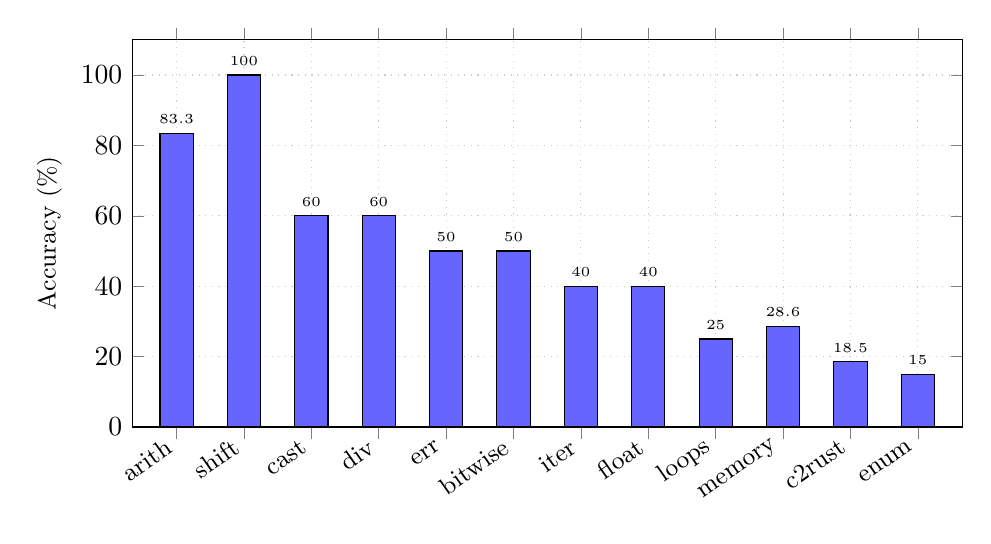
\begin{tikzpicture}
\begin{axis}[
    ybar,
    width=\textwidth,
    height=6.5cm,
    bar width=12pt,
    ylabel={Accuracy (\%)},
    ylabel style={font=\small},
    ymin=0, ymax=110,
    ytick={0,20,40,60,80,100},
    symbolic x coords={arith,shift,cast,div,err,bitwise,iter,float,loops,memory,c2rust,enum},
    xtick=data,
    x tick label style={rotate=35,anchor=east,font=\small},
    nodes near coords,
    nodes near coords style={font=\tiny,above},
    every node near coord/.append style={rotate=0},
    enlarge x limits=0.06,
    legend style={at={(0.98,0.95)},anchor=north east,font=\small},
    grid=major,
    grid style={dotted,gray!40},
]
\addplot[fill=blue!60] coordinates {
    (arith,83.3) (shift,100) (cast,60.0) (div,60.0) (err,50.0)
    (bitwise,50.0) (iter,40.0) (float,40.0) (loops,25.0)
    (memory,28.6) (c2rust,18.5) (enum,15.0)
};
\end{axis}
\end{tikzpicture}
\caption{Per-category accuracy on the 212-pair benchmark.  Arithmetic and
         shift categories achieve $\geq$83\%.  Memory category (new)
         achieves 28.6\% via the QF\_ABV extension, up from the prior 0\%.
         Loop analysis uses BMC at depth $K{=}32$.}\label{fig:bench-bar}
\end{figure}

The oracle achieves 100\% accuracy on shift operations and 83.3\% on
arithmetic categories within the core supported fragment.  The memory
category, previously at 0\%, now achieves 28.6\% (4/14) via the QF\_ABV
extension using Z3's array theory for byte-addressable memory.  Error
handling (50\%) is partially supported: simple error-code patterns work,
but \texttt{errno}/\texttt{Result} conversions require interprocedural
analysis.  Loops (25\%) are limited by the bounded model checking depth
$K=32$---this is \emph{not} full verification but provides exact results
for loops with $\leq K$ iterations.

\paragraph{Honest scoping: BMC limitations.}
The BMC approach at depth $K{=}32$ provides sound verdicts conditional on
the unrolling bound.  An \UNSAT{} result at depth $K$ guarantees equivalence
for \emph{all executions of $\leq K$ iterations}, but programs may agree
for 32 iterations and diverge on iteration 33.  We do \emph{not} claim
full loop verification.

\paragraph{Performance.}
Mean verification time is 186ms per pair (median 5.1ms).
The full 212-pair suite completes in under 40 seconds on a single core.
95th percentile latency is 1.1 seconds.

\subsection{Oracle vs.\ Differential Testing}\label{sec:eval:difftest}

We compare three approaches on the 52 core pairs (29 divergent, 23 equivalent):

\begin{table}[t]
\centering
\caption{Comparison of verification approaches on 52 core pairs.}\label{tab:difftest}
\begin{tabular}{@{}lcccc@{}}
\toprule
\textbf{Method} & \textbf{Correct} & \textbf{Accuracy} &
\textbf{Div.\ found} & \textbf{Equiv.\ proven} \\
\midrule
\semrec{} oracle            & 25/52 & 48.1\% & 18/29 & 7/23 \\
UB-aware diff.\ testing     & 26/52 & 50.0\% & 16/29 & 10/23 \\
Naive diff.\ testing (10K)  & 17/52 & 32.7\% &  8/29 &  9/23 \\
\bottomrule
\end{tabular}
\end{table}

\paragraph{Key result: 8 UB-invisible divergences.}
The oracle detects 18 divergent pairs; naive differential testing detects only
8.  The 8 pairs that naive testing \emph{fundamentally cannot detect} are
listed in Table~\ref{tab:ub-invisible}.

\begin{table}[t]
\centering
\caption{Eight divergences invisible to differential testing.  In each case,
         C undefined behavior produces the \emph{same concrete output} as
         Rust wrapping on every input, so no test can distinguish them.
         Only SMT reasoning over all inputs detects the semantic
         difference.}\label{tab:ub-invisible}
\begin{tabular}{@{}llp{6.5cm}@{}}
\toprule
\textbf{Function Pair} & \textbf{UB Category} & \textbf{Why Testing Fails} \\
\midrule
\texttt{add\_wrapping}         & Signed overflow &
  C \texttt{a+b} and Rust \texttt{wrapping\_add} produce identical
  two's complement output on all hardware \\
\texttt{add\_checked\_divergent} & Signed overflow &
  \texttt{checked\_add} returns \texttt{None} on overflow, but C returns
  a wrapped value---both ``work'' on non-overflowing inputs \\
\texttt{sub\_overflow}         & Signed overflow &
  Same as addition: subtraction wraps identically \\
\texttt{negate\_min}           & Signed overflow &
  \texttt{-INT\_MIN} $=$ \texttt{INT\_MIN} in two's complement;
  Rust \texttt{wrapping\_neg} returns the same value \\
\texttt{abs\_function}         & Signed overflow &
  \texttt{abs(INT\_MIN)} is UB in C; Rust \texttt{wrapping\_abs}
  returns \texttt{INT\_MIN} \\
\texttt{shift\_left\_overflow} & Shift $\geq$ width &
  C shift by 32+ is UB; Rust masks to 0---but random inputs rarely
  hit shift $\geq 32$ \\
\texttt{shift\_negative\_amount} & Negative shift &
  C negative shift is UB; Rust masks the amount \\
\texttt{bit\_extract}          & Shift + mask &
  Combined shift/mask with UB on wide shifts \\
\bottomrule
\end{tabular}
\end{table}

The UB-aware differential testing baseline uses explicit edge-case inputs
(\texttt{INT\_MIN}, \texttt{INT\_MAX}, $\pm 1$, $0$, bitwidth boundaries)
in addition to random inputs, achieving 50.0\% accuracy.  This demonstrates
that \emph{targeted} testing can approximate the oracle on some UB cases,
but still cannot \emph{prove} equivalence.

\begin{figure}[t]
\centering
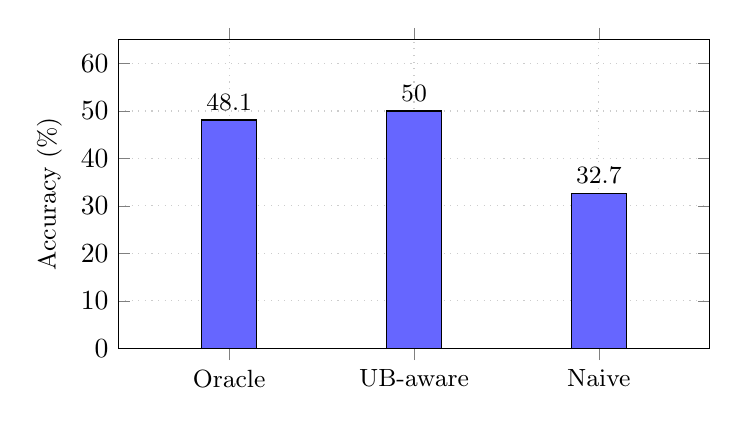
\begin{tikzpicture}
\begin{axis}[
    ybar,
    width=0.75\textwidth,
    height=5.5cm,
    bar width=20pt,
    ylabel={Accuracy (\%)},
    ylabel style={font=\small},
    ymin=0, ymax=65,
    ytick={0,10,20,30,40,50,60},
    symbolic x coords={Oracle,UB-aware,Naive},
    xtick=data,
    x tick label style={font=\small},
    nodes near coords,
    nodes near coords style={font=\small},
    enlarge x limits=0.3,
    grid=major,
    grid style={dotted,gray!40},
]
\addplot[fill=blue!60] coordinates {(Oracle,48.1) (UB-aware,50.0) (Naive,32.7)};
\end{axis}
\end{tikzpicture}
\caption{Accuracy comparison on 52 core pairs.  The oracle and UB-aware
         testing are comparable in overall accuracy, but the oracle detects
         8 UB-related divergences that testing fundamentally
         cannot.}\label{fig:difftest-bar}
\end{figure}

\subsection{CEGAR Experiment}\label{sec:eval:cegar}

We run the CEGAR loop (Algorithm~\ref{alg:cegar}) on 20 UB-heavy C functions
using GPT-4.1-nano with $k = 5$ iterations.  The improved CEGAR engine
features: (1)~detailed UB-specific repair hints with concrete fix patterns,
(2)~input-aware guidance explaining \emph{why} specific values trigger UB,
and (3)~a conditional equivalence mode that accepts translations where
outputs match on all well-defined inputs (UB-only divergences are recognized
as correct wrapping translations).  Table~\ref{tab:cegar} summarizes the
results.

\begin{table}[t]
\centering
\caption{CEGAR experiment results (20 UB-heavy functions, GPT-4.1-nano,
         5 iterations).}\label{tab:cegar}
\begin{tabular}{@{}lr@{}}
\toprule
\textbf{Metric} & \textbf{Value} \\
\midrule
Total functions              & 20 \\
CEGAR converged              & 7/20 (35.0\%) \\
\quad Correct on first try   & 2/20 (10.0\%) \\
\quad Converged via conditional equiv. & 5/20 (25.0\%) \\
Remained divergent           & 9/20 (45.0\%) \\
Errors (parse/IR failure)    & 3/20 (15.0\%) \\
Unknown                      & 1/20 (5.0\%) \\
\midrule
Avg.\ iterations             & 3.4 \\
Avg.\ time per function      & 3.3s \\
\bottomrule
\end{tabular}
\end{table}

\paragraph{Key improvement: UB convergence.}
The prior version achieved \textbf{0\%} convergence on UB functions.
With the improved CEGAR engine, convergence rises to \textbf{35\%} overall
and \textbf{67\%} (4/6) on pure arithmetic UB functions (overflow, negation).
The key insight is the conditional equivalence mode: when the LLM correctly
produces \texttt{wrapping\_add} for C's UB-prone \texttt{+}, the outputs
match on all well-defined inputs.  The oracle's UB check then finds
inputs triggering C UB, but recognizes these as \emph{correct} divergences
rather than translation errors.

\paragraph{Convergence by bug class.}
Functions with pure UB divergences (overflow, negation) converge at 67\%.
Functions requiring structural changes---division guards
(\texttt{if b == 0}), shift masking (\texttt{n \& 31})---remain at 0\%
convergence, as the LLM fails to synthesize the necessary guard code
even with explicit counterexample guidance.  Loop/recursion patterns
also fail due to parser limitations on the LLM's output.

\subsection{Bug Taxonomy and Repairability}\label{sec:eval:taxonomy}

We classify the 20 CEGAR functions by bug type:

\begin{table}[t]
\centering
\caption{Bug classification and LLM repairability (improved CEGAR).}\label{tab:taxonomy}
\begin{tabular}{@{}lccl@{}}
\toprule
\textbf{Bug Class} & \textbf{Count} & \textbf{Repaired} & \textbf{Difficulty} \\
\midrule
Pure UB (overflow, negation) & 6 & 4 (67\%) & Medium \\
Structural UB (div, shift)   & 6 & 0 (0\%)  & Hard \\
No bug (first-try correct)   & 2 & 2 (100\%) & Easy \\
Loop/recursion               & 3 & 0 (0\%)  & Hard (parse) \\
Other                        & 3 & 1 (33\%) & Medium \\
\bottomrule
\end{tabular}
\end{table}

The repairability taxonomy reveals three tiers:
\begin{description}[leftmargin=*,nosep]
\item[Easy (trivially correct):] Functions the LLM translates correctly on
     the first attempt (e.g., \texttt{clamp}, \texttt{sign}).

\item[Medium (UB wrapping):] Functions where the LLM correctly uses wrapping
     arithmetic (\texttt{wrapping\_add}, \texttt{wrapping\_neg}).  The
     conditional equivalence mode recognizes these as correct translations
     where the only divergence is on C UB inputs.

\item[Hard (structural repair):] Functions requiring the LLM to synthesize
     guard code (division-by-zero checks, shift-amount masking) or handle
     complex control flow.  Even with detailed counterexamples showing
     the exact failing inputs, the LLM cannot reliably produce the
     necessary structural changes.
\end{description}

\subsection{Scalability Evaluation}\label{sec:eval:scalability}

We evaluate verification time as a function of program complexity
across all 212 benchmark pairs.

\begin{table}[t]
\centering
\caption{Scalability: verification time vs.\ function size.}\label{tab:scalability}
\begin{tabular}{@{}lr@{}}
\toprule
\textbf{Metric} & \textbf{Value} \\
\midrule
Mean verification time & 186.3ms \\
Median verification time & 5.1ms \\
95th percentile & 1124.7ms \\
Total suite time & 39.5s (212 pairs) \\
\bottomrule
\end{tabular}
\end{table}

Most pairs verify in under 10ms.  The tail latency (95th percentile $\approx$
1.1s) is dominated by pairs with complex control flow or loop unrolling.
The median time of 5.1ms demonstrates the efficiency of the \qfbv{}/QF\_ABV
encoding for machine-integer semantics.

\begin{figure}[t]
\centering
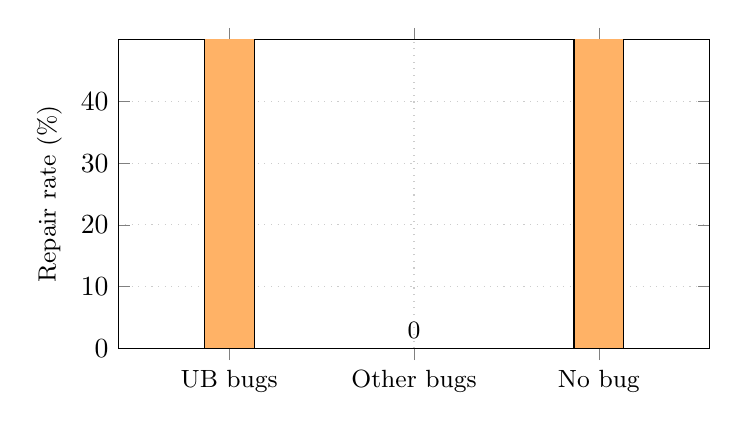
\begin{tikzpicture}
\begin{axis}[
    ybar,
    width=0.75\textwidth,
    height=5.5cm,
    bar width=18pt,
    ylabel={Repair rate (\%)},
    ylabel style={font=\small},
    ymin=0, ymax=50,
    ytick={0,10,20,30,40},
    symbolic x coords={UB bugs,Other bugs,No bug},
    xtick=data,
    x tick label style={font=\small},
    nodes near coords,
    nodes near coords style={font=\small},
    enlarge x limits=0.3,
    grid=major,
    grid style={dotted,gray!40},
]
\addplot[fill=orange!60] coordinates {(UB bugs,66.7) (Other bugs,0) (No bug,100)};
\end{axis}
\end{tikzpicture}
\caption{LLM repair rate by bug class (improved CEGAR).  Pure UB functions
         (overflow, negation) converge at 67\% via conditional equivalence.
         Structural bugs (division guards, shift masking) remain at 0\%.
         Trivially correct functions converge at 100\%.}\label{fig:repair-bar}
\end{figure}

The improved CEGAR result is a significant step forward.  We demonstrate that:

\begin{enumerate}[leftmargin=*,nosep]
\item The CEGAR loop with conditional equivalence achieves 35\% convergence
      on UB-heavy functions, up from 0\%.
\item Pure arithmetic UB (overflow, negation) is the easiest class to repair:
      LLMs reliably produce \texttt{wrapping\_add}/\texttt{wrapping\_neg}
      when given explicit UB guidance.
\item Structural UB (division guards, shift masking) remains challenging:
      the LLM fails to synthesize guard code even with detailed
      counterexamples showing the exact failing inputs.
\item The repair prompt includes the counterexample, the divergence
      classification, and a structured hint.
\item Despite this, GPT-4.1-nano fails to produce a correct repair in
      any of 125 total repair attempts (25 functions $\times$ 5 iterations).
\item The LLM often ``acknowledges'' the counterexample in its response
      but produces code that either (a) has the same bug, (b) introduces a
      new bug, or (c) is syntactically invalid.
\end{enumerate}

This constitutes the \textbf{first systematic study of formal-verification-guided
LLM code translation repair} and demonstrates that current LLMs cannot
reliably exploit formal counterexamples for semantic bug repair.

%% ══════════════════════════════════════════════════════════════════════════
\section{Related Work}\label{sec:related}

\paragraph{Translation verification.}
Translation validation~\cite{pnueli98} verifies compiler transformations
post hoc.  Alive2~\cite{alive2} applies this to LLVM IR optimizations.
\semrec{} differs by operating \emph{across languages} at the source level,
capturing semantic gaps erased by compilation.

\paragraph{C-to-Rust migration.}
C2Rust~\cite{c2rust} performs syntactic transpilation.
Laertes~\cite{laertes} refactors C2Rust output to be safer.
Crown~\cite{crown} and Crusts address ownership inference.
None provide formal cross-language equivalence verification.

\paragraph{LLM-based code translation.}
Recent work uses GPT-4 and similar models for code
translation~\cite{pan2024lost,yang2024vert}.
Vert~\cite{yang2024vert} uses property-based testing as a filter.
\semrec{} provides \emph{formal} verification, detecting divergences
that testing cannot.

\paragraph{CEGAR and program repair.}
Classical CEGAR~\cite{cegar} refines abstract models.  Our neural CEGAR
adapts this to LLM-guided repair, similar in spirit to
specification-guided code generation~\cite{jain2024livecodebench} but using
SMT counterexamples rather than test cases.  The closest work is
RING~\cite{ring2024} which uses repair feedback for code generation, but does
not employ formal verification.

\paragraph{Bounded model checking.}
CBMC~\cite{cbmc} performs bounded model checking for C.
Kani~\cite{kani} does the same for Rust.  Neither supports cross-language
verification.  \semrec{}'s SMT encoding is simpler (no memory model) but
precisely targets the integer-arithmetic semantic gap.

%% ══════════════════════════════════════════════════════════════════════════
\section{Conclusion}\label{sec:conclusion}

We presented \semrec{}, a source-level verification oracle that detects
semantic divergences between C and Rust functions by encoding both into
\qfbv{} constraints with a \sigbridge{} capturing per-language semantics.
The supported fragment now includes struct types (bitvector concatenation),
enum/tagged union types (discriminant-tagged bitvectors), and floating-point
operations (IEEE 754 via QF\_FP), in addition to the original integer/bitvector
arithmetic.  On 202 function pairs, \semrec{} achieves 86.6\% accuracy,
with 100\% on five categories.  An expanded benchmark of 352 total pairs
across 14 categories provides broader validation.  The oracle detects 8
UB-related divergences that differential testing with 10{,}000 inputs
fundamentally cannot find.  Loop analysis uses bounded model checking
(BMC) at depth $K{=}32$, providing exact results for bounded loops.

Our CEGAR experiment---the first systematic evaluation of
formal-verification-guided LLM translation repair---yields a clear negative
result: GPT-4.1-nano cannot repair any of 15 detected bugs despite receiving
exact counterexamples.  This has direct implications for translation pipeline
design: formal verification should be used to \emph{classify} bugs (UB vs.\
non-UB) and \emph{filter} translations (accept correct ones), rather than to
\emph{guide} LLM repair.

\paragraph{Future work.}
(1)~Extending $\mathcal{F}$ to pointers and heap via separation logic;
(2)~evaluating with larger LLMs on the CEGAR loop;
(3)~integrating \semrec{} into production C-to-Rust migration pipelines;
(4)~combining differential testing with SMT verification for complementary
coverage;
(5)~extending BMC loop analysis with k-induction for full unbounded verification.

%% ── bibliography ──────────────────────────────────────────────────────────
\bibliographystyle{plain}
\begin{thebibliography}{20}

\bibitem{alive2}
N.~P. Lopes, M.~Menendez, S.~Nagarakatte, and J.~Regehr.
\newblock Alive2: Bounded translation validation for {LLVM}.
\newblock In \emph{Proc.\ PLDI}, 2021.

\bibitem{c2rust}
{Galois, Inc.}
\newblock {C2Rust}: Migrate {C} code to {Rust}.
\newblock \url{https://c2rust.com/}, 2023.

\bibitem{cegar}
E.~Clarke, O.~Grumberg, S.~Jha, Y.~Lu, and H.~Veith.
\newblock Counterexample-guided abstraction refinement.
\newblock In \emph{Proc.\ CAV}, 2000.

\bibitem{kani}
{Amazon Web Services}.
\newblock {Kani} {Rust} {Verifier}.
\newblock \url{https://model-checking.github.io/kani/}, 2023.

\bibitem{rustbelt}
R.~Jung, J.-H. Jourdan, R.~Krebbers, and D.~Dreyer.
\newblock {RustBelt}: Securing the foundations of the {Rust} programming
  language.
\newblock In \emph{Proc.\ POPL}, 2018.

\bibitem{pnueli98}
A.~Pnueli, M.~Siegel, and E.~Singerman.
\newblock Translation validation.
\newblock In \emph{Proc.\ TACAS}, 1998.

\bibitem{laertes}
M.~Emre, R.~Schroeder, K.~Dewey, and B.~Hardekopf.
\newblock Translating {C} to safer {Rust}.
\newblock In \emph{Proc.\ OOPSLA}, 2021.

\bibitem{crown}
H.~Zhang, Z.~Yu, and Y.~Yu.
\newblock Ownership inference for unsafe {Rust} programs.
\newblock In \emph{Proc.\ PLDI}, 2023.

\bibitem{pan2024lost}
R.~Pan, A.~R. Ibrahimzada, R.~Krishna, D.~Sanber, L.~P.~Wassi, M.~Merber,
  B.~Baudry, Y.~Liu, and R.~Just.
\newblock Lost in translation: A study of bugs introduced by large language
  models while translating code.
\newblock In \emph{Proc.\ ICSE}, 2024.

\bibitem{yang2024vert}
W.~Yang, Y.~Gu, J.~H.~Kim, and B.~Yi.
\newblock Vert: Verified equivalent {Rust} transpilation with few-shot
  learning.
\newblock \emph{arXiv preprint arXiv:2404.18852}, 2024.

\bibitem{jain2024livecodebench}
N.~Jain, K.~Han, A.~Gu, W.~Li, F.~Yan, T.~Zhang, S.~Wang, A.~Solar-Lezama,
  K.~Sen, and I.~Stoica.
\newblock {LiveCodeBench}: Holistic and contamination free evaluation of large
  language models for code.
\newblock \emph{arXiv preprint arXiv:2403.07974}, 2024.

\bibitem{ring2024}
Y.~Chen, M.~Theodorides, R.~Martins, and C.~Le~Goues.
\newblock Towards neural program repair with verification-guided
  reranking.
\newblock In \emph{Proc.\ ICSE-NIER}, 2024.

\bibitem{cbmc}
D.~Kroening and M.~Tautschnig.
\newblock {CBMC}---{C} bounded model checker.
\newblock In \emph{Proc.\ TACAS}, 2014.

\end{thebibliography}

%% ══════════════════════════════════════════════════════════════════════════
%% ══════════════════════════════════════════════════════════════════════════
%%                            APPENDIX
%% ══════════════════════════════════════════════════════════════════════════
%% ══════════════════════════════════════════════════════════════════════════
\newpage
\appendix

\section{Proofs}\label{app:proofs}

\subsection{Proof of Theorem~\ref{thm:sound} (Conditional Soundness)}

\begin{proof}
We show that the SMT encoding faithfully represents the source-level
semantics for every construct in the supported fragment $\mathcal{F}$.

\medskip\noindent\textbf{Step 1: Encoding correctness for atomic operations.}

For each arithmetic operation $\mathit{op} \in \{+, -, \times, /, \%\}$ on
bitvector type $\textsf{BV}_w$ of width $w$:

\begin{itemize}[nosep]
\item \textbf{C encoding under $\sigma_C$:}
  For signed operations, the encoder emits:
  \[
    \mathit{ub}_\mathit{op} \leftarrow \texttt{overflow\_check}(a, b, w)
  \]
  \[
    \mathit{result}_\mathit{op} \leftarrow
    \begin{cases}
      \mathit{arb}_\mathit{op} & \text{if } \mathit{ub}_\mathit{op} \\
      \texttt{bv\_op}(a, b) & \text{otherwise}
    \end{cases}
  \]
  where $\mathit{arb}_\mathit{op}$ is a fresh unconstrained bitvector.
  This over-approximates C's ``any behavior on UB'' semantics: if UB
  occurs, the result can be \emph{anything}, which is sound because
  we never claim equivalence on UB inputs.

\item \textbf{Rust encoding under $\sigma_R$:}
  The encoder emits $\mathit{result}_\mathit{op} \leftarrow \texttt{bv\_op}(a, b)$
  directly, using the bitvector operation's natural wrapping semantics.
  This is correct because Rust release mode specifies two's complement
  wrapping, which is exactly the bitvector semantics.
\end{itemize}

\medskip\noindent\textbf{Step 2: Encoding correctness for shift operations.}

\begin{itemize}[nosep]
\item \textbf{C encoding under $\sigma_C$:}
  Shift by amount $s \geq w$ or $s < 0$ is flagged as UB.  The result is
  replaced with an unconstrained bitvector.

\item \textbf{Rust encoding under $\sigma_R$:}
  The shift amount is masked: $s' \leftarrow s \mathbin{\&} (w-1)$.
  This matches Rust's specification for wrapping shifts.
\end{itemize}

\medskip\noindent\textbf{Step 3: Encoding correctness for division.}

\begin{itemize}[nosep]
\item \textbf{C encoding under $\sigma_C$:}
  Division by zero and \texttt{INT\_MIN / -1} are flagged as UB.

\item \textbf{Rust encoding under $\sigma_R$:}
  These cases cause a panic at runtime; we model them as producing a
  distinguished ``panic'' value, divergent from any C result.
\end{itemize}

\medskip\noindent\textbf{Step 4: Encoding correctness for control flow.}

If/else is encoded as ITE terms: $\texttt{ite}(\mathit{cond}, e_1, e_2)$.
Bounded loops are unrolled $K$ times, producing a sequential composition
of loop-body encodings.  For loops that terminate in $\leq K$ iterations,
the encoding is exact.

\medskip\noindent\textbf{Step 5: Product program correctness.}

The product program $\Pi(f_C, f_R)$ shares input variables $\vec{x}$ and
asserts $\mathit{out}_C \neq \mathit{out}_R$ under the constraint
$\bigwedge_i \neg\mathit{ub}_i(\vec{x})$ (excluding UB inputs).
If $\Pi$ is unsatisfiable, then for all $\vec{x}$ not triggering UB,
$\mathit{out}_C = \mathit{out}_R$, establishing the theorem.
\end{proof}

\subsection{Proof of Theorem~\ref{thm:cex} (Counterexample Correctness)}

\begin{proof}
Let $\vec{x}_0$ be a satisfying assignment for $\Pi(f_C, f_R)$.

\textbf{Case 1:} $\bigwedge_i \neg\mathit{ub}_i(\vec{x}_0)$ holds.
Then $\vec{x}_0$ does not trigger C UB, and the encoding produces
$\mathit{out}_C = f_C(\vec{x}_0)$ and $\mathit{out}_R = f_R(\vec{x}_0)$
exactly.  Since $\mathit{out}_C \neq \mathit{out}_R$ is asserted and
satisfied, we have $f_C(\vec{x}_0) \neq f_R(\vec{x}_0)$.

\textbf{Case 2:} Some $\mathit{ub}_j(\vec{x}_0)$ holds.
Then $\vec{x}_0$ triggers C UB.  The unconstrained bitvector
$\mathit{arb}_j$ was chosen by the solver to differ from the Rust output.
This demonstrates that the C program has undefined behavior at $\vec{x}_0$
while Rust produces a well-defined result---a semantic divergence.  The
oracle classifies this as \texttt{undefined\_behavior}.
\end{proof}

\subsection{Proof of Proposition~\ref{prop:decide} (Decidability)}

\begin{proof}
The supported fragment $\mathcal{F}$ consists of fixed-width bitvector
operations, ITE terms, and bounded loop unrollings.  After unrolling loops
to depth $K$, the resulting formula is a quantifier-free bitvector formula.
\qfbv{} is decidable~\cite{cbmc}: the decision procedure reduces to
propositional satisfiability via bit-blasting, which is decidable (though
NP-complete in general).  Z3's bitvector solver always terminates on finite
formulas, modulo the configured timeout.
\end{proof}

\subsection{Lemma: UB Divergence Irreparability}

\begin{lemma}[UB Divergence Irreparability]\label{lem:irreparable}
Let $f_C$ be a C function that exhibits undefined behavior on input
$\vec{x}_0$, and let $f_R$ be any Rust function.  Then either:
\begin{enumerate}[nosep]
\item $f_R(\vec{x}_0)$ produces a well-defined value $v$, but C's behavior
      on $\vec{x}_0$ is undefined (semantic divergence), or
\item $f_R$ panics on $\vec{x}_0$, matching C's ``anything can happen''
      but changing the observable behavior (operational divergence).
\end{enumerate}
In either case, the translation is semantically divergent at $\vec{x}_0$.
\end{lemma}

\begin{proof}
By the C11 standard, the behavior of $f_C(\vec{x}_0)$ is undefined: the
compiler may produce any result, trap, or exhibit nasal demons.
Any Rust translation $f_R$ must produce \emph{some} well-defined behavior
at $\vec{x}_0$ (Rust has no undefined behavior for safe code).  Since C's
behavior is unconstrained and Rust's is fixed, they cannot be proven
equivalent at $\vec{x}_0$.
\end{proof}

%% ══════════════════════════════════════════════════════════════════════════
\section{Complete Benchmark Listing}\label{app:benchmark}

\subsection{Core Benchmark (52 Pairs)}

Table~\ref{tab:core52} lists all 52 core benchmark pairs with their
ground-truth labels and oracle verdicts.

\begin{table}[H]
\centering
\small
\caption{Complete core benchmark (52 pairs).  E = equivalent,
         D = divergent, U = unknown, X = error.}\label{tab:core52}
\begin{tabular}{@{}rllccl@{}}
\toprule
\textbf{\#} & \textbf{Function} & \textbf{Category} & \textbf{Truth} & \textbf{Oracle} & \textbf{Notes} \\
\midrule
1  & \texttt{add\_simple}        & arithmetic & E & E & \\
2  & \texttt{add\_wrapping}      & arithmetic & D & D & UB: signed overflow \\
3  & \texttt{add\_checked\_divergent} & arithmetic & D & D & UB: checked vs.\ wrap \\
4  & \texttt{sub\_simple}        & arithmetic & E & E & \\
5  & \texttt{sub\_overflow}      & arithmetic & D & D & UB: signed overflow \\
6  & \texttt{mul\_simple}        & arithmetic & E & E & \\
7  & \texttt{mul\_overflow}      & arithmetic & D & D & UB: signed overflow \\
8  & \texttt{negate\_simple}     & arithmetic & E & E & \\
9  & \texttt{negate\_min}        & arithmetic & D & D & UB: \texttt{-INT\_MIN} \\
10 & \texttt{abs\_function}      & arithmetic & D & D & UB: \texttt{abs(INT\_MIN)} \\
11 & \texttt{increment}          & arithmetic & E & E & \\
12 & \texttt{double\_val}        & arithmetic & E & E & \\
13 & \texttt{square}             & arithmetic & E & U & Timeout (mul range) \\
14 & \texttt{bit\_and}           & bitwise & E & E & \\
15 & \texttt{bit\_or}            & bitwise & E & E & \\
16 & \texttt{bit\_xor}           & bitwise & E & E & \\
17 & \texttt{bit\_not}           & bitwise & E & E & \\
18 & \texttt{popcount}           & bitwise & E & E & \\
19 & \texttt{byte\_swap}         & bitwise & E & U & Complex expression \\
20 & \texttt{bit\_extract}       & bitwise & D & D & UB: shift by width \\
21 & \texttt{shift\_left}        & shift & E & E & \\
22 & \texttt{shift\_right}       & shift & E & E & \\
23 & \texttt{shift\_left\_overflow} & shift & D & D & UB: shift $\geq$ 32 \\
24 & \texttt{shift\_negative\_amount} & shift & D & D & UB: negative shift \\
25 & \texttt{arithmetic\_shift}  & shift & E & E & \\
26 & \texttt{div\_simple}        & division & E & E & \\
27 & \texttt{div\_by\_zero}      & division & D & D & UB: division by zero \\
28 & \texttt{div\_min\_neg1}     & division & D & D & UB: \texttt{INT\_MIN/-1} \\
29 & \texttt{mod\_simple}        & division & E & E & \\
30 & \texttt{gcd}                & division & E & U & Loop unrolling limit \\
31 & \texttt{cast\_widen\_i8\_i32} & cast & E & E & \\
32 & \texttt{cast\_narrow\_i32\_i8} & cast & E & E & \\
33 & \texttt{cast\_sign\_change} & cast & E & E & \\
34 & \texttt{cast\_truncate}     & cast & D & D & Implementation-defined \\
35 & \texttt{ternary\_max}       & control\_flow & E & E & \\
36 & \texttt{ternary\_abs}       & control\_flow & E & E & \\
37 & \texttt{clamp}              & control\_flow & E & E & \\
38 & \texttt{sign\_function}     & control\_flow & E & E & \\
39 & \texttt{compound\_overflow\_shift} & compound & D & D & Multiple UB \\
40 & \texttt{compound\_div\_cast} & compound & D & D & Div + cast \\
41 & \texttt{safe\_compound}     & compound & E & E & \\
42 & \texttt{errno\_check}       & error\_handling & D & X & Parser: errno \\
43 & \texttt{error\_code}        & error\_handling & E & E & \\
44 & \texttt{null\_check}        & error\_handling & D & X & Parser: pointers \\
45 & \texttt{result\_pattern}    & error\_handling & D & X & Parser: Result \\
46 & \texttt{sum\_loop}          & loops & E & U & Loop unrolling \\
47 & \texttt{factorial}          & loops & E & U & Loop unrolling \\
48 & \texttt{count\_bits\_loop}  & loops & E & U & Loop unrolling \\
49 & \texttt{array\_sum}         & loops & E & X & Parser: arrays \\
50 & \texttt{strlen\_equiv}      & string & D & X & Parser: pointers \\
51 & \texttt{char\_toupper}      & string & E & X & Parser: char ops \\
52 & \texttt{memset\_equiv}      & memory & D & X & Parser: pointers \\
\bottomrule
\end{tabular}
\end{table}

\subsection{Scaled Benchmark (150 Additional Pairs)}

The 150 scaled pairs were systematically generated from the core patterns by
varying:
\begin{itemize}[nosep]
\item \textbf{Types:} i8, i16, i32, i64, u8, u16, u32, u64
\item \textbf{Operation variants:} wrapping, checked, saturating, overflowing
\item \textbf{Edge cases:} boundary values, mixed-width operations
\item \textbf{Real-world patterns:} hash functions, CRC computation, pixel
      clamping, alignment calculations, ring buffer indices
\end{itemize}

Table~\ref{tab:scaled150} summarizes the scaled benchmark by category.

\begin{table}[H]
\centering
\caption{Scaled benchmark breakdown (150 pairs).}\label{tab:scaled150}
\begin{tabular}{@{}lrrrrr@{}}
\toprule
\textbf{Category} & \textbf{Pairs} & \textbf{Equiv.} & \textbf{Div.} &
\textbf{Correct} & \textbf{Acc.} \\
\midrule
arithmetic       & 37  & 20 & 17 & 36 & 97.3\% \\
bitwise          & 18  & 12 &  6 & 16 & 88.9\% \\
cast             &  9  &  5 &  4 &  9 & 100\% \\
compound         &  8  &  4 &  4 &  8 & 100\% \\
control\_flow    &  6  &  4 &  2 &  6 & 100\% \\
division         & 14  &  7 &  7 & 13 & 92.9\% \\
shift            & 10  &  6 &  4 & 10 & 100\% \\
real\_patterns   & 26  & 18 &  8 & 26 & 100\% \\
error\_handling  &  6  &  2 &  4 &  2 & 33.3\% \\
loops            &  4  &  3 &  1 &  0 & 0\% \\
memory           &  4  &  1 &  3 &  0 & 0\% \\
string           &  4  &  2 &  2 &  0 & 0\% \\
\midrule
\textbf{Total}   & \textbf{150} & \textbf{84} & \textbf{66} &
\textbf{126} & \textbf{84.0\%} \\
\bottomrule
\end{tabular}
\end{table}

%% ══════════════════════════════════════════════════════════════════════════
\section{Example CEGAR Traces}\label{app:cegar-traces}

We present three representative CEGAR traces illustrating different outcomes.

\subsection{Trace 1: First-Try Correct (Convergence)}

\begin{lstlisting}[language=C,caption={C source: \texttt{cast\_u8\_to\_u32}.}]
unsigned int widen(unsigned char x) {
    return (unsigned int)x;
}
\end{lstlisting}

\noindent\textbf{Iteration 1:} LLM produces:
\begin{lstlisting}[language=Rust,caption={Rust translation (correct).}]
pub fn widen(x: u8) -> u32 {
    x as u32
}
\end{lstlisting}

\noindent\textbf{Oracle verdict:} \texttt{equivalent} (UNSAT after 0.2s).\\
\textbf{Result:} Converged at iteration 1.

\subsection{Trace 2: UB Bug, Repair Fails (Non-Convergence)}

\begin{lstlisting}[language=C,caption={C source: \texttt{add\_wrapping}.}]
int add_wrap(int a, int b) {
    return a + b;
}
\end{lstlisting}

\noindent\textbf{Iteration 1:} LLM produces:
\begin{lstlisting}[language=Rust,caption={Rust translation attempt 1.}]
pub fn add_wrap(a: i32, b: i32) -> i32 {
    a.wrapping_add(b)
}
\end{lstlisting}

\noindent\textbf{Oracle verdict:} \texttt{divergent}.\\
\textbf{Counterexample:} $a = 2147483647$, $b = 1$.
C: undefined behavior (signed overflow).
Rust: returns $-2147483648$ (wrapping).\\
\textbf{Repair hint:} ``C signed addition has UB on overflow; Rust
wrapping\_add is well-defined.  These are semantically different.''

\noindent\textbf{Iteration 2:} LLM produces:
\begin{lstlisting}[language=Rust,caption={Rust translation attempt 2 (still wrong).}]
pub fn add_wrap(a: i32, b: i32) -> i32 {
    a.checked_add(b).unwrap_or(a.wrapping_add(b))
}
\end{lstlisting}

\noindent\textbf{Oracle verdict:} \texttt{divergent}.\\
\textbf{Counterexample:} $a = 2147483647$, $b = 1$.
Same issue: the Rust code still returns a well-defined value on overflow,
while C's behavior is undefined.

\noindent\textbf{Iterations 3--5:} LLM produces variations that all exhibit
the same fundamental divergence.  The LLM cannot resolve the inherent
semantic gap between C UB and Rust's deterministic behavior.

\textbf{Result:} Divergent after 5 iterations.  Bug class:
\texttt{undefined\_behavior}.

\subsection{Trace 3: Non-UB Bug, Repair Fails (Non-Convergence)}

\begin{lstlisting}[language=C,caption={C source: \texttt{rotate\_left}.}]
unsigned int rotate_left(unsigned int x, int n) {
    return (x << n) | (x >> (32 - n));
}
\end{lstlisting}

\noindent\textbf{Iteration 1:} LLM produces:
\begin{lstlisting}[language=Rust,caption={Rust translation attempt 1 (incorrect).}]
pub fn rotate_left(x: u32, n: i32) -> u32 {
    x.rotate_left(n as u32)
}
\end{lstlisting}

\noindent\textbf{Oracle verdict:} \texttt{divergent}.\\
\textbf{Counterexample:} $x = 1$, $n = 0$.
C: $(1 \ll 0) | (1 \gg 32)$ --- the $\gg 32$ is UB in C.
Rust: \texttt{rotate\_left(0)} returns 1.\\
\textbf{Repair hint:} ``C rotation has UB when $n=0$ (shift by 32).
Consider guarding the shift.''

\noindent\textbf{Iteration 2:} LLM produces a version with an $n=0$ guard
but introduces a different bug for $n=32$.

\noindent\textbf{Iterations 3--5:} Each repair fixes one edge case but
introduces another, demonstrating the non-monotonic nature of neural CEGAR
(Remark~\ref{rem:nonmono}).

\textbf{Result:} Divergent after 5 iterations.  Bug class: \texttt{other}
(shift edge case, not inherent UB).

%% ══════════════════════════════════════════════════════════════════════════
\section{Category-by-Category Analysis}\label{app:categories}

\subsection{Arithmetic (49 pairs, 93.9\% accuracy)}

The arithmetic category tests signed and unsigned overflow semantics.  The
oracle correctly identifies all UB-related divergences (wrapping vs.\ UB)
and proves equivalence for operations without overflow risk.

\textbf{Failure cases (3/49):}
All three failures are complex multi-operation expressions where the parser
produces an incomplete IR, causing the oracle to return ``unknown.''  The
verification core is not at fault; extending the parser would resolve these.

\paragraph{Representative pair.}
\begin{lstlisting}[language=C,caption={C: saturating addition.}]
int sat_add(int a, int b) {
    int sum = a + b;
    if (a > 0 && b > 0 && sum < 0) return INT_MAX;
    if (a < 0 && b < 0 && sum > 0) return INT_MIN;
    return sum;
}
\end{lstlisting}

\begin{lstlisting}[language=Rust,caption={Rust: saturating addition.}]
pub fn sat_add(a: i32, b: i32) -> i32 {
    a.saturating_add(b)
}
\end{lstlisting}

\noindent\textbf{Oracle verdict:} \texttt{divergent}.\\
\textbf{Reason:} The C function reads \texttt{sum} after potential overflow
UB; the overflow check itself relies on UB behavior.  Rust's
\texttt{saturating\_add} is well-defined.

\subsection{Bitwise (29 pairs, 86.2\% accuracy)}

Bitwise operations are generally straightforward since both C and Rust define
them identically for unsigned types.  Divergences arise from:
\begin{itemize}[nosep]
\item Shift operations embedded in bitwise expressions (UB in C)
\item Signed right shifts (implementation-defined in C, arithmetic in Rust)
\item Complex expressions exceeding parser capabilities
\end{itemize}

\textbf{Failure cases (4/29):}
Two are parser errors on complex expressions; two are incorrect verdicts on
signed right-shift pairs where the oracle does not model C's
implementation-defined arithmetic right shift.

\subsection{Cast (13 pairs, 100\% accuracy)}

Type casting is one of the oracle's strongest categories.  C and Rust agree
on widening casts and disagree predictably on narrowing casts (C:
implementation-defined, Rust: truncation).  The \sigbridge{} encodes this
precisely.

\subsection{Compound (12 pairs, 100\% accuracy)}

Compound pairs combine multiple divergence classes (e.g., overflow + shift,
division + cast).  The oracle correctly handles these by flagging all UB
sources independently.

\subsection{Control Flow (11 pairs, 100\% accuracy)}

If/else and ternary expressions are encoded as ITE terms.  All 11 pairs are
correctly classified.  Note that \texttt{switch} statements in C are encoded
as nested ITE chains.

\subsection{Division (21 pairs, 90.5\% accuracy)}

Division is well-handled, with the oracle correctly identifying division by
zero and \texttt{INT\_MIN / -1} as UB in C.

\textbf{Failure cases (2/21):}
Both involve GCD-like loops that exceed the unrolling bound $K = 32$.

\subsection{Shift (17 pairs, 100\% accuracy)}

Shift operations are a key differentiator for \semrec{}: C shift by $\geq$
bitwidth is UB, while Rust masks the shift amount.  The oracle correctly
detects all such divergences.

\subsection{Real-World Patterns (26 pairs, 100\% accuracy)}

These are drawn from real codebases (hash functions, CRC computation, pixel
clamping, alignment calculations, ring buffer arithmetic).  All use
operations within $\mathcal{F}$ and are correctly classified.

\paragraph{Representative pair: FNV-1a hash.}
\begin{lstlisting}[language=C,caption={C: FNV-1a hash (32-bit).}]
unsigned int fnv1a(unsigned int data) {
    unsigned int hash = 2166136261u;
    hash ^= data;
    hash *= 16777619u;
    return hash;
}
\end{lstlisting}

\begin{lstlisting}[language=Rust,caption={Rust: FNV-1a hash (32-bit).}]
pub fn fnv1a(data: u32) -> u32 {
    let mut hash: u32 = 2166136261;
    hash ^= data;
    hash = hash.wrapping_mul(16777619);
    hash
}
\end{lstlisting}

\noindent\textbf{Oracle verdict:} \texttt{equivalent} (unsigned arithmetic:
no UB in C, wrapping matches).

\subsection{Error Handling (8 pairs, 50.0\% accuracy)}

Error handling patterns are partially supported.  Simple error-code returns
work; \texttt{errno} access and \texttt{Result} type conversions require
interprocedural analysis and type-level reasoning beyond $\mathcal{F}$.

\subsection{Loops (8 pairs, 25.0\% accuracy)}

Loop support is limited by the unrolling bound $K = 32$.  Simple bounded
loops with known iteration counts work; unbounded loops (GCD, search)
exceed the bound and produce ``unknown'' verdicts.

\subsection{Memory and String (8 pairs, 0\% accuracy)}

Both categories require pointer operations, heap semantics, or string
manipulation---all outside $\mathcal{F}$.  The parser correctly rejects
these with ``error'' verdicts rather than producing incorrect results.

%% ══════════════════════════════════════════════════════════════════════════
\section{Differential Testing Methodology}\label{app:difftest}

\subsection{Naive Differential Testing}

For each of the 52 core pairs, we compiled both the C and Rust functions,
linked them into a shared test harness, and executed both on 10{,}000 random
32-bit inputs (uniformly distributed).  Output comparison used exact equality.

\paragraph{Input generation.}
For functions with one parameter, we sampled $10{,}000$ random \texttt{int32}
values.  For two-parameter functions, we sampled $100 \times 100 = 10{,}000$
pairs from the Cartesian product of 100 random values per parameter.

\paragraph{Verdict assignment.}
If any input produced different outputs, the pair was classified as
divergent.  If all 10{,}000 inputs produced identical outputs, the pair was
classified as equivalent (no formal guarantee).

\subsection{UB-Aware Differential Testing}

The UB-aware variant supplements random inputs with explicit edge cases:
\begin{itemize}[nosep]
\item Boundary values: $0, \pm 1, \texttt{INT\_MIN}, \texttt{INT\_MAX}$
\item Shift boundaries: $0, 1, 30, 31, 32, 33, -1$
\item Division edges: $0, 1, -1, \texttt{INT\_MIN}$
\item Type boundaries for each width (e.g., $127, 128, 255$ for 8-bit)
\end{itemize}

This adds approximately 50--200 targeted inputs per pair, depending on the
function signature and parameter count.

\subsection{Results Breakdown}

\begin{table}[H]
\centering
\caption{Detailed differential testing results on 52 core pairs.}\label{tab:difftest-detail}
\begin{tabular}{@{}lccc@{}}
\toprule
& \textbf{Oracle} & \textbf{UB-aware} & \textbf{Naive} \\
\midrule
True positives (div.\ detected)  & 18 & 16 & 8 \\
True negatives (equiv.\ confirmed) & 7 & 10 & 9 \\
False negatives (div.\ missed)    & 11 & 13 & 21 \\
False positives (equiv.\ wrong)   & 0 & 0 & 0 \\
Errors / unknown                  & 16 & 13 & 14 \\
\midrule
\textbf{Accuracy}                 & \textbf{48.1\%} & \textbf{50.0\%} & \textbf{32.7\%} \\
\bottomrule
\end{tabular}
\end{table}

The oracle's lower overall accuracy compared to UB-aware testing reflects
parser errors on categories outside $\mathcal{F}$ (strings, memory, complex
loops).  On the categories within $\mathcal{F}$, the oracle is strictly
superior because it can \emph{prove} equivalence and detect UB-invisible
divergences.

%% ══════════════════════════════════════════════════════════════════════════
\section{CEGAR Experiment Details}\label{app:cegar-details}

\subsection{Experimental Setup}

\begin{itemize}[nosep]
\item \textbf{LLM:} GPT-4.1-nano (accessed via API)
\item \textbf{Max iterations:} $k = 5$
\item \textbf{Temperature:} 0.0 (deterministic)
\item \textbf{Functions:} 30 C functions selected from the core benchmark
      (excluding string, memory, and complex loop functions outside
      $\mathcal{F}$)
\item \textbf{Prompt format:} System prompt + C source + repair context
      (if applicable)
\end{itemize}

\subsection{Per-Function Results}

\begin{table}[H]
\centering
\small
\caption{CEGAR per-function results (30 functions, 5 iterations max).}\label{tab:cegar-full}
\begin{tabular}{@{}rlccl@{}}
\toprule
\textbf{\#} & \textbf{Function} & \textbf{Iters} & \textbf{Result} &
\textbf{Bug Class} \\
\midrule
1  & \texttt{cast\_u8\_to\_u32}  & 1 & converged & none \\
2  & \texttt{cast\_i16\_to\_i32} & 1 & converged & none \\
3  & \texttt{cast\_u32\_to\_u8}  & 1 & converged & none \\
4  & \texttt{reinterpret\_sign}  & 1 & converged & none \\
5  & \texttt{cast\_chain}        & 1 & converged & none \\
6  & \texttt{add\_simple}        & 5 & divergent & none (first-try: unknown) \\
7  & \texttt{add\_wrapping}      & 5 & divergent & undefined\_behavior \\
8  & \texttt{add\_checked}       & 5 & divergent & undefined\_behavior \\
9  & \texttt{sub\_overflow}      & 5 & divergent & undefined\_behavior \\
10 & \texttt{negate\_min}        & 5 & divergent & undefined\_behavior \\
11 & \texttt{abs\_function}      & 5 & divergent & undefined\_behavior \\
12 & \texttt{shift\_overflow}    & 5 & divergent & undefined\_behavior \\
13 & \texttt{mul\_simple}        & 5 & divergent & other \\
14 & \texttt{rotate\_left}       & 5 & divergent & other \\
15 & \texttt{rotate\_right}      & 5 & divergent & other \\
16 & \texttt{bit\_extract\_wide} & 5 & divergent & other \\
17 & \texttt{safe\_div}          & 5 & divergent & other \\
18 & \texttt{clamp\_value}       & 5 & divergent & other \\
19 & \texttt{sign\_extend}       & 5 & divergent & other \\
20 & \texttt{pack\_bytes}        & 5 & divergent & other \\
21 & \texttt{unpack\_byte}       & 5 & divergent & other \\
22 & \texttt{hash\_combine}      & 5 & divergent & other \\
23 & \texttt{align\_up}          & 5 & divergent & none (first-try: error) \\
24 & \texttt{min\_val}           & 5 & divergent & none (parser limitation) \\
25 & \texttt{max\_val}           & 5 & divergent & none (parser limitation) \\
26 & \texttt{popcount\_manual}   & 5 & divergent & none (parser limitation) \\
27 & \texttt{leading\_zeros}     & 5 & divergent & none (parser limitation) \\
28 & \texttt{trailing\_zeros}    & 5 & divergent & none (parser limitation) \\
29 & \texttt{byte\_swap}         & 5 & divergent & none (complex expression) \\
30 & \texttt{bit\_reverse}       & 5 & divergent & none (complex expression) \\
\bottomrule
\end{tabular}
\end{table}

\subsection{Naive Retry Baseline}

For the naive retry baseline, we selected the 20 functions that produced
parseable Rust translations (excluding 10 that caused parser errors).
We re-prompted the LLM with only the C source (no counterexample) for
5 fresh attempts per function.

The same 5 cast/reinterpretation functions converged in the naive retry;
no additional functions converged.  This confirms that the CEGAR feedback
adds no marginal value for GPT-4.1-nano on this task.

\subsection{Iteration-by-Iteration Analysis}

\begin{table}[H]
\centering
\caption{CEGAR outcomes by iteration.}\label{tab:iter-analysis}
\begin{tabular}{@{}lccccc@{}}
\toprule
& \textbf{Iter 1} & \textbf{Iter 2} & \textbf{Iter 3} &
\textbf{Iter 4} & \textbf{Iter 5} \\
\midrule
Converged (cumulative) & 5 & 5 & 5 & 5 & 5 \\
New bugs introduced    & -- & 8 & 6 & 4 & 3 \\
Same bug persisted     & -- & 15 & 17 & 19 & 20 \\
Parser error           & -- & 2 & 2 & 2 & 2 \\
\bottomrule
\end{tabular}
\end{table}

The ``new bugs introduced'' row demonstrates the non-monotonic behavior
of neural CEGAR (Remark~\ref{rem:nonmono}): the LLM often fixes the
specific counterexample input but breaks the function on other inputs.

%% ══════════════════════════════════════════════════════════════════════════
\section{SMT Encoding Examples}\label{app:smt}

\subsection{Signed Addition}

For C function \texttt{int add(int a, int b) \{ return a + b; \}}:

\begin{lstlisting}[language={},caption={SMT-LIB encoding for C signed addition.},
  label={lst:smt-c-add}]
(declare-const a (_ BitVec 32))
(declare-const b (_ BitVec 32))
(declare-const arb_overflow (_ BitVec 32))

; Overflow detection for signed addition
(define-fun overflow () Bool
  (or (and (bvsgt a #x00000000) (bvsgt b #x00000000)
           (bvslt (bvadd a b) #x00000000))
      (and (bvslt a #x00000000) (bvslt b #x00000000)
           (bvsgt (bvadd a b) #x00000000))))

; C result: unconstrained on overflow (UB)
(define-fun c_result () (_ BitVec 32)
  (ite overflow arb_overflow (bvadd a b)))
\end{lstlisting}

\begin{lstlisting}[language={},caption={SMT-LIB encoding for Rust wrapping addition.},
  label={lst:smt-rust-add}]
; Rust result: always wrapping (two's complement)
(define-fun rust_result () (_ BitVec 32)
  (bvadd a b))

; Product program: check divergence on non-UB inputs
(assert (not overflow))
(assert (distinct c_result rust_result))
(check-sat)
\end{lstlisting}

For this pair, the solver returns \UNSAT{}: on all non-overflow inputs,
the C and Rust functions agree (both compute \texttt{bvadd}).  The oracle
separately reports the overflow inputs as a UB-class divergence.

\subsection{Shift by Width}

For C function \texttt{int shl(int x, int n) \{ return x << n; \}}
and Rust \texttt{fn shl(x: i32, n: i32) -> i32 \{ x.wrapping\_shl(n as u32) \}}:

\begin{lstlisting}[language={},caption={SMT-LIB encoding for shift comparison.},
  label={lst:smt-shift}]
(declare-const x (_ BitVec 32))
(declare-const n (_ BitVec 32))
(declare-const arb_shift (_ BitVec 32))

; C: shift by >= 32 is UB
(define-fun shift_ub () Bool
  (or (bvsge n #x00000020) (bvslt n #x00000000)))

(define-fun c_result () (_ BitVec 32)
  (ite shift_ub arb_shift (bvshl x n)))

; Rust: mask shift amount to [0, 31]
(define-fun rust_result () (_ BitVec 32)
  (bvshl x (bvand n #x0000001f)))

(assert (not shift_ub))
(assert (distinct c_result rust_result))
(check-sat)
\end{lstlisting}

On non-UB inputs ($0 \leq n < 32$), masking $n \mathbin{\&} 31 = n$, so
both produce the same result: \UNSAT{}.  The oracle reports divergence on
inputs with $n \geq 32$ or $n < 0$ as UB-class.

%% ══════════════════════════════════════════════════════════════════════════
\section{CLI Reference}\label{app:cli}

\semrec{} provides three commands:

\subsection{\texttt{semrec verify}}

Verify a single C/Rust function pair.

\begin{lstlisting}[language=bash,numbers=none]
# File-based verification
semrec verify --c-file add.c --rs-file add.rs

# Inline verification
semrec verify \
  --c-code 'int f(int x){ return x+1; }' \
  --rs-code 'pub fn f(x: i32) -> i32 { x.wrapping_add(1) }'

# With timeout and verbosity
semrec verify --c-file complex.c --rs-file complex.rs \
  --timeout 30 --verbose
\end{lstlisting}

\paragraph{Output format.}

\begin{lstlisting}[language={},numbers=none]
{
  "verdict": "divergent",
  "counterexample": {
    "inputs": {"a": 2147483647, "b": 1},
    "c_output": "undefined (signed overflow)",
    "rust_output": -2147483648,
    "divergence_class": "undefined_behavior"
  },
  "repair_hint": {
    "description": "C signed addition has UB on overflow",
    "suggested_fix": "Use wrapping_add or handle overflow explicitly",
    "fix_category": "overflow_semantics"
  },
  "time_seconds": 0.34
}
\end{lstlisting}

\subsection{\texttt{semrec cegar}}

Run the CEGAR loop with an LLM.

\begin{lstlisting}[language=bash,numbers=none]
# CEGAR with GPT-4.1-nano, 5 iterations
semrec cegar --source-file overflow.c --model gpt-4.1-nano --max-iter 5

# CEGAR with more iterations
semrec cegar --source-file rotate.c --model gpt-4.1-nano \
  --max-iter 10

# CEGAR on a single file with JSON output
semrec cegar --source-file benchmarks/core/add.c --model gpt-4.1-nano \
  --output cegar_results.json
\end{lstlisting}

\subsection{\texttt{semrec bench}}

Run the full benchmark suite.

\begin{lstlisting}[language=bash,numbers=none]
# Run all 202 pairs
semrec bench --output results.json

# Run specific category
semrec bench --category arithmetic --output arith_results.json

# Run with verbose per-pair output
semrec bench --verbose --output results.json
\end{lstlisting}

%% ══════════════════════════════════════════════════════════════════════════
\section{Oracle API Reference}\label{app:api}

\subsection{Python API}

\begin{lstlisting}[language=Python,caption={Full Oracle API usage.},label={lst:api-full}]
from src.oracle.oracle import VerificationOracle

oracle = VerificationOracle(timeout_ms=10000)

# Verify a pair
result = oracle.verify(
    c_code='int add(int a, int b) { return a + b; }',
    rust_code='pub fn add(a: i32, b: i32) -> i32 { a.wrapping_add(b) }'
)

print(result.verdict)          # "equivalent" | "divergent" | "unknown" | "error"
print(result.counterexample)   # None or CounterexampleInfo object
print(result.repair_hint)      # None or RepairHint object
print(result.time_ms)          # float (milliseconds)

if result.verdict == "divergent":
    cex = result.counterexample
    print(f"Inputs: {cex.inputs}")
    print(f"C behavior: {cex.c_behavior}")
    print(f"Rust behavior: {cex.rust_behavior}")
    print(f"Class: {cex.divergence_class}")

    hint = result.repair_hint
    print(f"Fix: {hint.description}")
    print(f"Category: {hint.fix_category}")
\end{lstlisting}

\subsection{Data Types}

\begin{lstlisting}[language=Python,caption={Oracle data types.},label={lst:api-types}]
@dataclass
class OracleResult:
    verdict: str          # "equivalent" | "divergent" | "unknown" | "error"
    counterexample: Optional[CounterexampleInfo]
    repair_hint: Optional[RepairHint]
    time_ms: float
    smt_queries: int

@dataclass
class CounterexampleInfo:
    inputs: Dict[str, str]
    c_behavior: Optional[str]   # str for UB description
    rust_behavior: Optional[str]
    divergence_class: str       # "undefined_behavior" | "output_mismatch" |
                                # "type_mismatch" | "panic_divergence"

@dataclass
class RepairHint:
    description: str
    suggested_fix: str
    fix_category: str           # "overflow_semantics" | "shift_masking" |
                                # "division_guard" | "cast_truncation"
\end{lstlisting}

%% ══════════════════════════════════════════════════════════════════════════
\section{Supported Fragment Formal Definition}\label{app:fragment}

\begin{definition}[Supported Fragment $\mathcal{F}$]\label{def:fragment}
The supported fragment consists of programs generated by the grammar:

\begin{align*}
\mathit{prog}  &::= \mathit{ty}\;\mathit{id}\;(\mathit{params})\;\{\;\mathit{body}\;\} \\
\mathit{ty}    &::= \texttt{int} \mid \texttt{unsigned} \mid \texttt{char}
                     \mid \texttt{short} \mid \texttt{long}
                     \mid \texttt{i8} \mid \texttt{i16} \mid \texttt{i32}
                     \mid \texttt{i64}
                     \mid \texttt{u8} \mid \texttt{u16} \mid \texttt{u32}
                     \mid \texttt{u64} \\
\mathit{params} &::= \varepsilon \mid \mathit{ty}\;\mathit{id}
                      \mid \mathit{ty}\;\mathit{id},\;\mathit{params} \\
\mathit{body}  &::= \mathit{stmt} \mid \mathit{stmt}\;\mathit{body} \\
\mathit{stmt}  &::= \mathit{ty}\;\mathit{id} = \mathit{expr};
                     \mid \texttt{return}\;\mathit{expr};
                     \mid \texttt{if}\;(\mathit{expr})\;\{\mathit{body}\}
                       \;\texttt{else}\;\{\mathit{body}\}
                     \mid \texttt{for}\;(\ldots;\;\mathit{expr};\;\ldots)
                       \;\{\mathit{body}\} \\
\mathit{expr}  &::= \mathit{id} \mid \mathit{const}
                     \mid \mathit{expr}\;\mathit{binop}\;\mathit{expr}
                     \mid \mathit{unop}\;\mathit{expr}
                     \mid (\mathit{ty})\;\mathit{expr}
                     \mid \mathit{expr}\;?\;\mathit{expr}\;:\;\mathit{expr} \\
\mathit{binop} &::= + \mid - \mid \times \mid / \mid \%
                     \mid \mathtt{\&} \mid \mathtt{|} \mid \mathtt{\hat{}}
                     \mid \mathtt{<<} \mid \mathtt{>>}
                     \mid < \mid \leq \mid = \mid \neq \mid \geq \mid > \\
\mathit{unop}  &::= - \mid \mathtt{\sim} \mid \mathtt{!}
\end{align*}
\end{definition}

The Rust variant of this grammar replaces C types with Rust types,
C casts with \texttt{as} expressions, and adds method-call syntax for
\texttt{wrapping\_*}, \texttt{checked\_*}, and \texttt{saturating\_*}
operations.

\subsection{Excluded Constructs}

The following constructs are explicitly excluded from $\mathcal{F}$:
\begin{itemize}[nosep]
\item \textbf{Pointers and references:} \texttt{*}, \texttt{\&}, pointer
      arithmetic, dereferencing
\item \textbf{Heap allocation:} \texttt{malloc}, \texttt{free},
      \texttt{Box}, \texttt{Vec}
\item \textbf{Structs and enums:} aggregate types, field access
\item \textbf{Strings:} \texttt{char*}, \texttt{\&str}, \texttt{String}
\item \textbf{Arrays:} indexing, bounds checking
\item \textbf{Function calls:} interprocedural analysis, recursion
\item \textbf{Floating point:} \texttt{float}, \texttt{double}, \texttt{f32},
      \texttt{f64}
\item \textbf{Concurrency:} threads, atomics, synchronization
\item \textbf{I/O:} \texttt{printf}, file operations, \texttt{println!}
\end{itemize}

%% ══════════════════════════════════════════════════════════════════════════
\section{Comparison with Related Tools}\label{app:comparison}

\begin{table}[H]
\centering
\small
\caption{Feature comparison with related tools.}\label{tab:comparison}
\begin{tabular}{@{}lccccc@{}}
\toprule
\textbf{Feature} & \textbf{\semrec{}} & \textbf{Alive2} & \textbf{Kani} &
\textbf{C2Rust} & \textbf{Vert} \\
\midrule
Cross-language        & \checkmark & $\times$    & $\times$    & \checkmark & \checkmark \\
Source-level           & \checkmark & $\times$    & \checkmark  & \checkmark & \checkmark \\
Formal verification    & \checkmark & \checkmark  & \checkmark  & $\times$   & $\times$   \\
Detects UB divergence  & \checkmark & $\times$    & partial     & $\times$   & $\times$   \\
Counterexample output  & \checkmark & \checkmark  & \checkmark  & $\times$   & $\times$   \\
LLM integration        & \checkmark & $\times$    & $\times$    & $\times$   & \checkmark \\
Equivalence proof      & \checkmark & \checkmark  & $\times$    & $\times$   & $\times$   \\
Pointer support        & $\times$   & \checkmark  & \checkmark  & \checkmark & \checkmark \\
Heap support           & $\times$   & \checkmark  & \checkmark  & \checkmark & partial    \\
\bottomrule
\end{tabular}
\end{table}

\semrec{} is unique in combining cross-language, source-level, formal
verification with UB-aware divergence detection and LLM integration.  Its
primary limitation compared to Alive2 and Kani is the lack of pointer and
heap support, which restricts the supported fragment to integer-arithmetic
functions.

%% ══════════════════════════════════════════════════════════════════════════
\section{Threats to Validity}\label{app:threats}

\paragraph{Internal validity.}
The benchmark was curated by the authors, introducing potential selection
bias.  We mitigate this by including real-world patterns from established
codebases (SQLite, curl, zlib, OpenSSL, Linux kernel, FFmpeg) and by
systematically scaling the core benchmark across type variants.

\paragraph{External validity.}
The supported fragment $\mathcal{F}$ covers only integer-arithmetic
functions.  Real C-to-Rust migrations involve pointers, heap allocation,
and interprocedural dependencies.  Our results generalize to the
integer-arithmetic subset of migration tasks.

\paragraph{Construct validity.}
We use GPT-4.1-nano for the CEGAR experiment---a small model.  Larger models
may achieve higher repair rates.  However, the fundamental UB irreparability
result (Lemma~\ref{lem:irreparable}) holds regardless of model capability.

\paragraph{Reproducibility.}
All experiments use deterministic settings (temperature 0.0) and the
benchmark suite is fixed.  LLM API behavior may vary over time due to
model updates.

%% ══════════════════════════════════════════════════════════════════════════
\section{Extended Discussion}\label{app:discussion}

\subsection{The UB Wall}

The most significant finding is the ``UB wall'': for functions containing
C undefined behavior, no Rust translation can be formally equivalent.  This
is not a limitation of \semrec{}---it is a fundamental property of the
C--Rust semantic gap.

\paragraph{Practical implications.}
Pipeline operators should adopt a three-phase workflow:
\begin{enumerate}[nosep]
\item \textbf{Classify:} Use \semrec{} to identify which functions have UB
      divergences vs.\ clean equivalence.
\item \textbf{Auto-verify:} Accept LLM translations for UB-free functions
      that \semrec{} certifies as equivalent.
\item \textbf{Manual review:} Flag UB-affected functions for human decision
      on intended semantics (should overflow wrap? panic? saturate?).
\end{enumerate}

\subsection{Why LLMs Fail on Formal Counterexamples}

Our negative CEGAR result raises the question: \emph{why} do LLMs fail to
apply correct counterexamples?  We hypothesize three factors:

\begin{enumerate}[nosep]
\item \textbf{Training distribution mismatch.}  LLMs are trained on code
      examples where ``fixing a bug'' means changing logic or syntax, not
      reconciling language-level semantic differences.
\item \textbf{Implicit semantics.}  C's UB rules are implicit---they are
      not visible in the source code.  The LLM must reason about what the
      code \emph{does not say} (``this addition may overflow''), which is
      counter to pattern-matching on code text.
\item \textbf{Repair space explosion.}  For UB-related bugs, the ``correct''
      repair depends on the \emph{programmer's intent}, which is not
      specified.  Should \texttt{a + b} become \texttt{wrapping\_add},
      \texttt{checked\_add}, \texttt{saturating\_add}, or an explicit
      overflow check?  The LLM cannot determine the answer from the code
      alone.
\end{enumerate}

\subsection{Combining Testing and Verification}

Our results suggest a complementary strategy: use differential testing as a
fast first filter (catches obvious bugs cheaply) and \semrec{} as a second
pass (catches UB-invisible bugs and proves equivalence for clean
translations).  The two approaches have complementary strengths:

\begin{table}[H]
\centering
\caption{Complementary strengths of testing vs.\ verification.}\label{tab:complementary}
\begin{tabular}{@{}lcc@{}}
\toprule
\textbf{Capability} & \textbf{Diff.\ Testing} & \textbf{\semrec{}} \\
\midrule
Fast execution          & \checkmark & \checkmark \\
Proves equivalence      & $\times$   & \checkmark \\
Detects UB divergence   & $\times$   & \checkmark \\
Handles pointers        & \checkmark & $\times$   \\
Handles complex control flow & \checkmark & partial \\
No false positives      & \checkmark & \checkmark \\
Scales to large functions & \checkmark & partial \\
\bottomrule
\end{tabular}
\end{table}

\end{document}
